\documentclass[12pt]{article}
\usepackage[english]{babel}
\usepackage[numbers]{natbib}
\usepackage{graphicx}
\usepackage{sectsty}
\usepackage{float}
\usepackage[table]{xcolor}
\usepackage{tabularx}
\usepackage{arydshln}

\bibliographystyle{apalike}
\setcitestyle{open={[},close={]}}
\sectionfont{\color{DarkBlue}} 
\subsectionfont{\color{LightBlue}}
\subsubsectionfont{\color{LightBlue}}
\paragraphfont{\color{LightBlue}}
\subparagraphfont{\color{LightBlue}}
\setlength{\arrayrulewidth}{1pt}
\renewcommand{\arraystretch}{1.5}
\newcolumntype{Y}{>{\centering\arraybackslash}X}
\definecolor{dkgreen}{rgb}{0,0.6,0}
\definecolor{gray}{rgb}{0.5,0.5,0.5}
\definecolor{mauve}{rgb}{0.58,0,0.82}
\definecolor{nicegreen}{rgb}{0.58, 0.98, 0.71}

\begin{document}
\definecolor{DarkBlue}{HTML}{4a5a8a} 
\definecolor{LightBlue}{HTML}{4f81bf}
\begin{titlepage}
    \begin{flushleft}
        \vspace{1cm} \Huge  \textbf{Cretaceous Gardens Controller}\\
        \vspace{1cm} \Huge  \textit{Software Architecture Design}\\
        \vspace{1cm} \Large \textit{SAD Version 2.0}\\
        \vspace{5cm} \LARGE         Team \#3\\ 
                                    12 November 2019
        \vfill       \Huge  \textbf{CS 460 Software Engineering}
    \end{flushleft}
\end{titlepage}
\normalsize 
\tableofcontents
\pagebreak

\section{Introduction} \label{intro}
\paragraph{} Good software is identified by the end user for its features and functionality, by the client
for its profitability and maintainability, and by the programmer for its legibility and clarity. It should be clear
that all three pillars ultimately characterize good software, but more importantly that the three are interdependent.
The developer must therefore guarantee all of the above for the sake of all entities involved. A top down approach has been
followed thus far. The Technical Feasibility Study posited and answered the fundamental question: Can it be done? The Requirements
Definition Document was then passed the baton and answered the next question: Within what parameters can it be done? Then, 
the Software Requirements Specification document sought to answer: What is the desired behavior of the system? Now this document 
seeks to answer the following: What design will guarantee the desired behavior in a manner that is clear, maintainable, extensible, 
and pragmatic?

\paragraph{} The ultimate goal is to ensure an efficient, safe, and maintainable implementation of the Cretaceous Gardens Controller 
(CGC) software. To that end, all objects are illustrated in their proper contexts, and their crucial 
functions have been delineated as clearly as possible while simultaneously allowing the programmer enough flexibility so 
as to not stifle his or her creative process. 

\paragraph{} This document is a road map for the eventual implementation of the system and details the most 
relevant objects and their relationships in the form of diagrams. Explanations accompany all diagrams for the sake of clarity.
Section \ref{over} presents an overview of the intended design, with descriptions of the largest subsystems that compose the CGC. 
Section \ref{specs} provides greater detail with respect to the individual components and their sub components. Section \ref{samp} 
provides a number of use cases for the system, which have been classified into a few categories. Section \ref{cons} delineates 
constraints to which the design is subject. Section \ref{defs} closes the document with the definitions of any terms used 
throughout the document that may need further clarification. 
\footnote{Introduction by Ezequiel Ramos.}.

\section{Design Overview} \label{over}
\paragraph{} The class architecture presented here aims to maximize efficiency, maintainability, and 
safety. Without an efficient system, it's safety may be compromised due to unnecessary 
delays between components. Maintainability can impact a safe implementation of the 
system if the system is permeable to programmer errors. The decoupling of concerns and 
a solid hierarchy are paramount \footnote{Diagrams by Siri and Anas.}.


\begin{figure}[H]
    \centerline{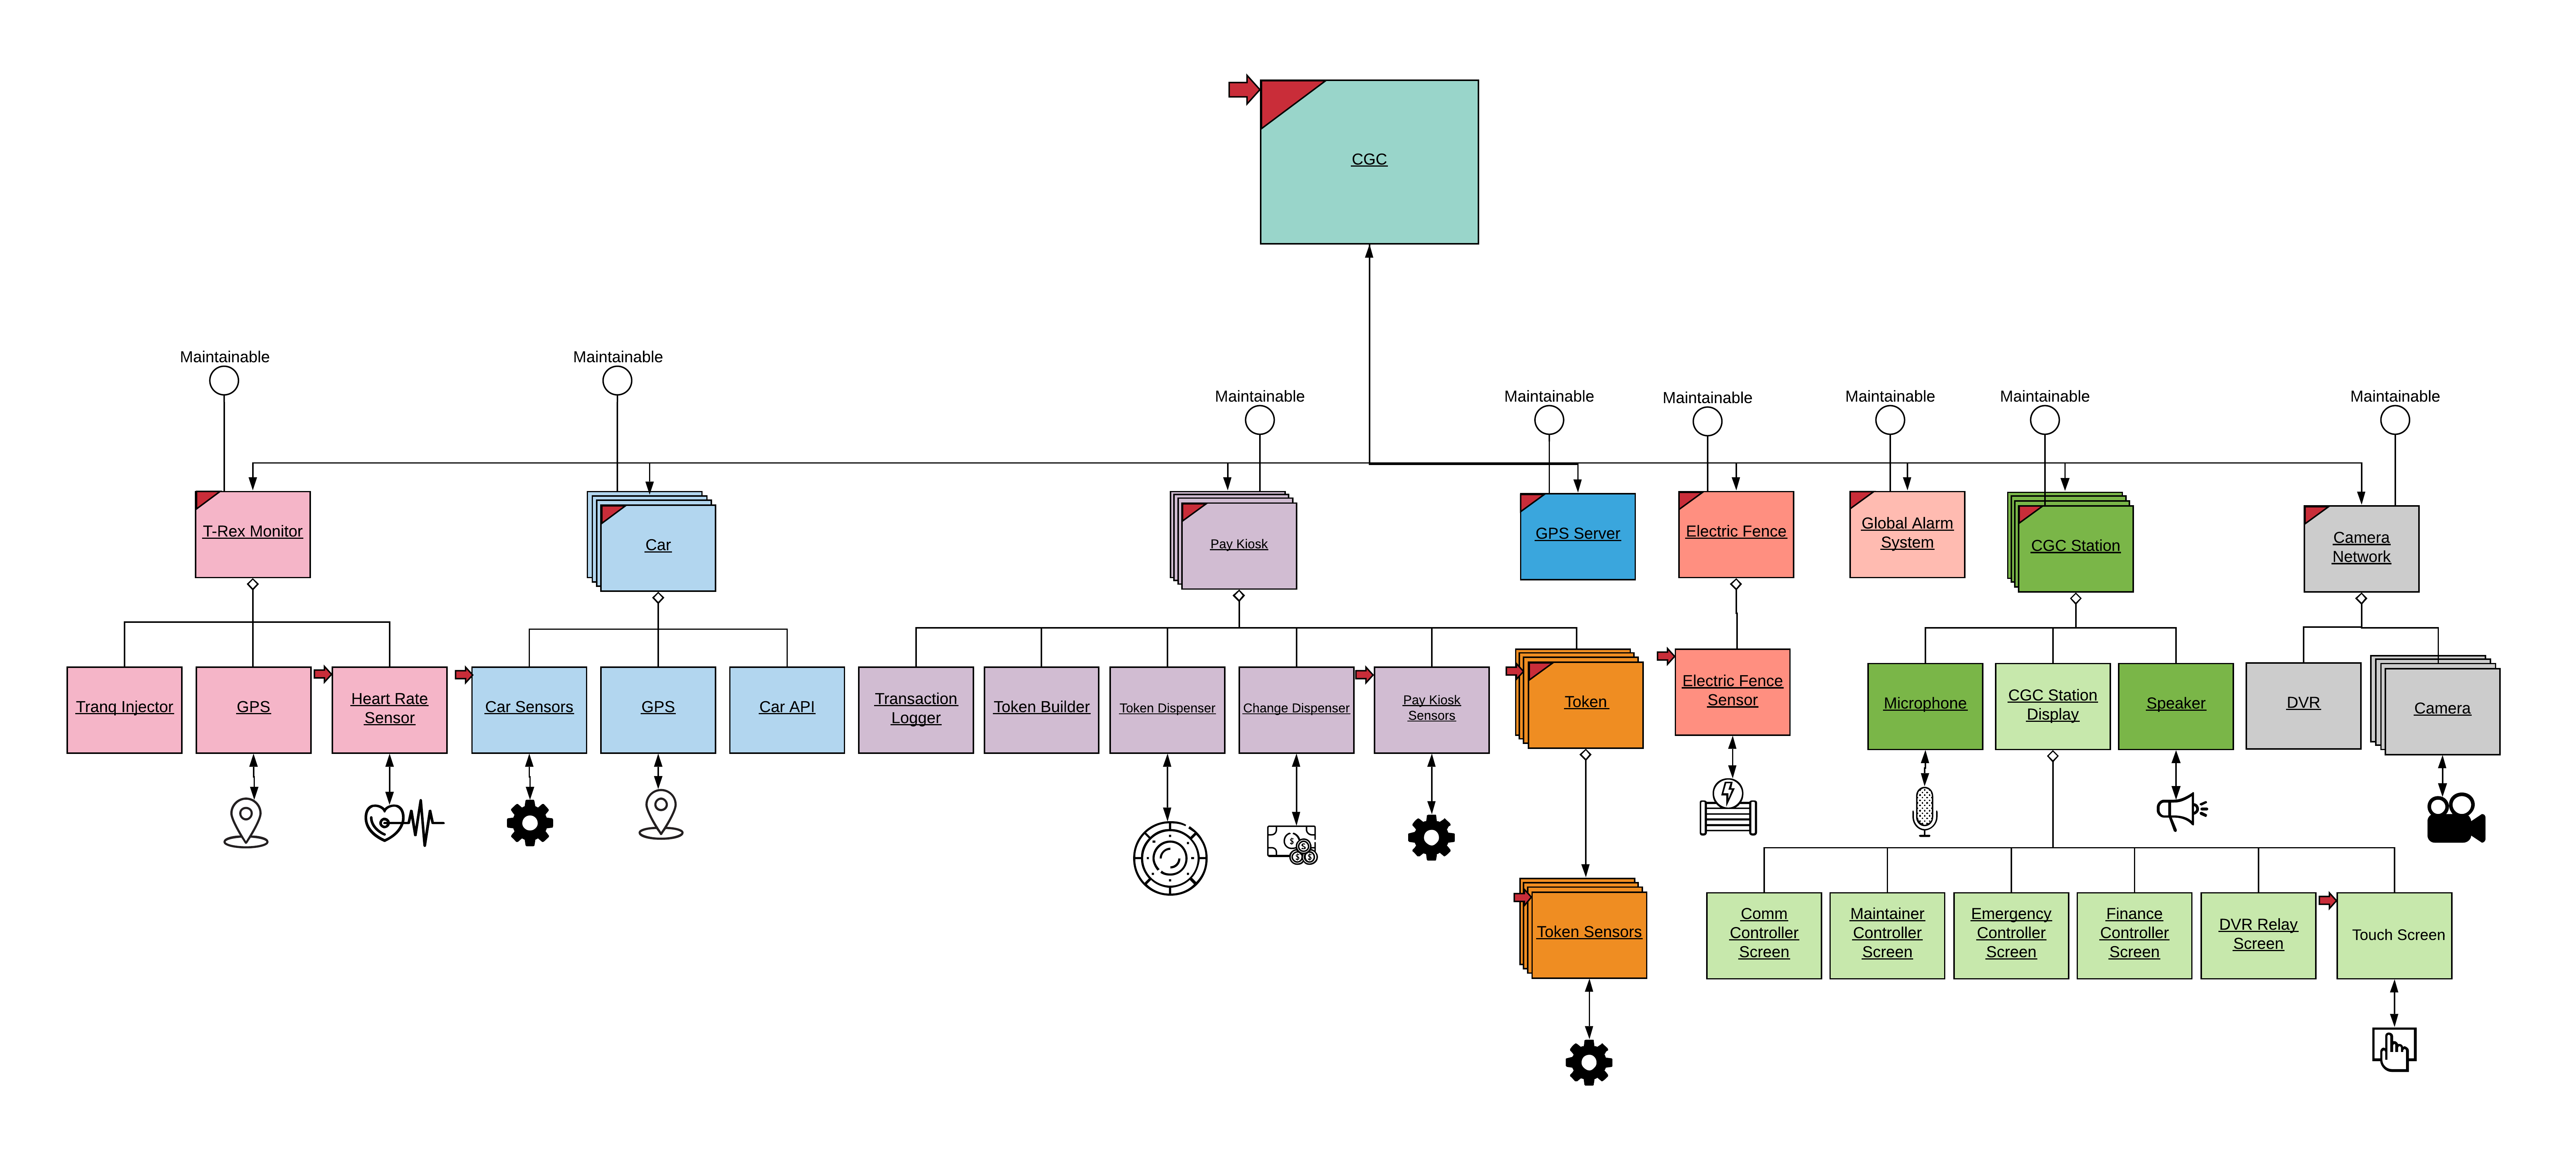
\includegraphics[scale=.095]{CGCOverview.png}}
    \caption{\textbf{CGC Overview:} This showcases the entire system as a whole working togethor. The CGC 
acts as a central system that can communicate with all active systems. We see it is not composed 
of any other objects, but rather it owns references to all active systems and helps keep track of 
them and helps bridge connections to other active systems. It is important to note that the red 
triangle in the corner of some objects symbolize that it runs in it's own thread. The red arrows 
symbolize that these objects can cause triggering events that generate some sort of action inside the 
system. One last thing that may seem unusual is the small circles above some objects labeled 
maintainable. This means that these objects implement the interface maintainable and the behavior 
associated with it.}
  \label{fig:CGCOverview}
\end{figure}    



\begin{figure}[H]
    \centerline{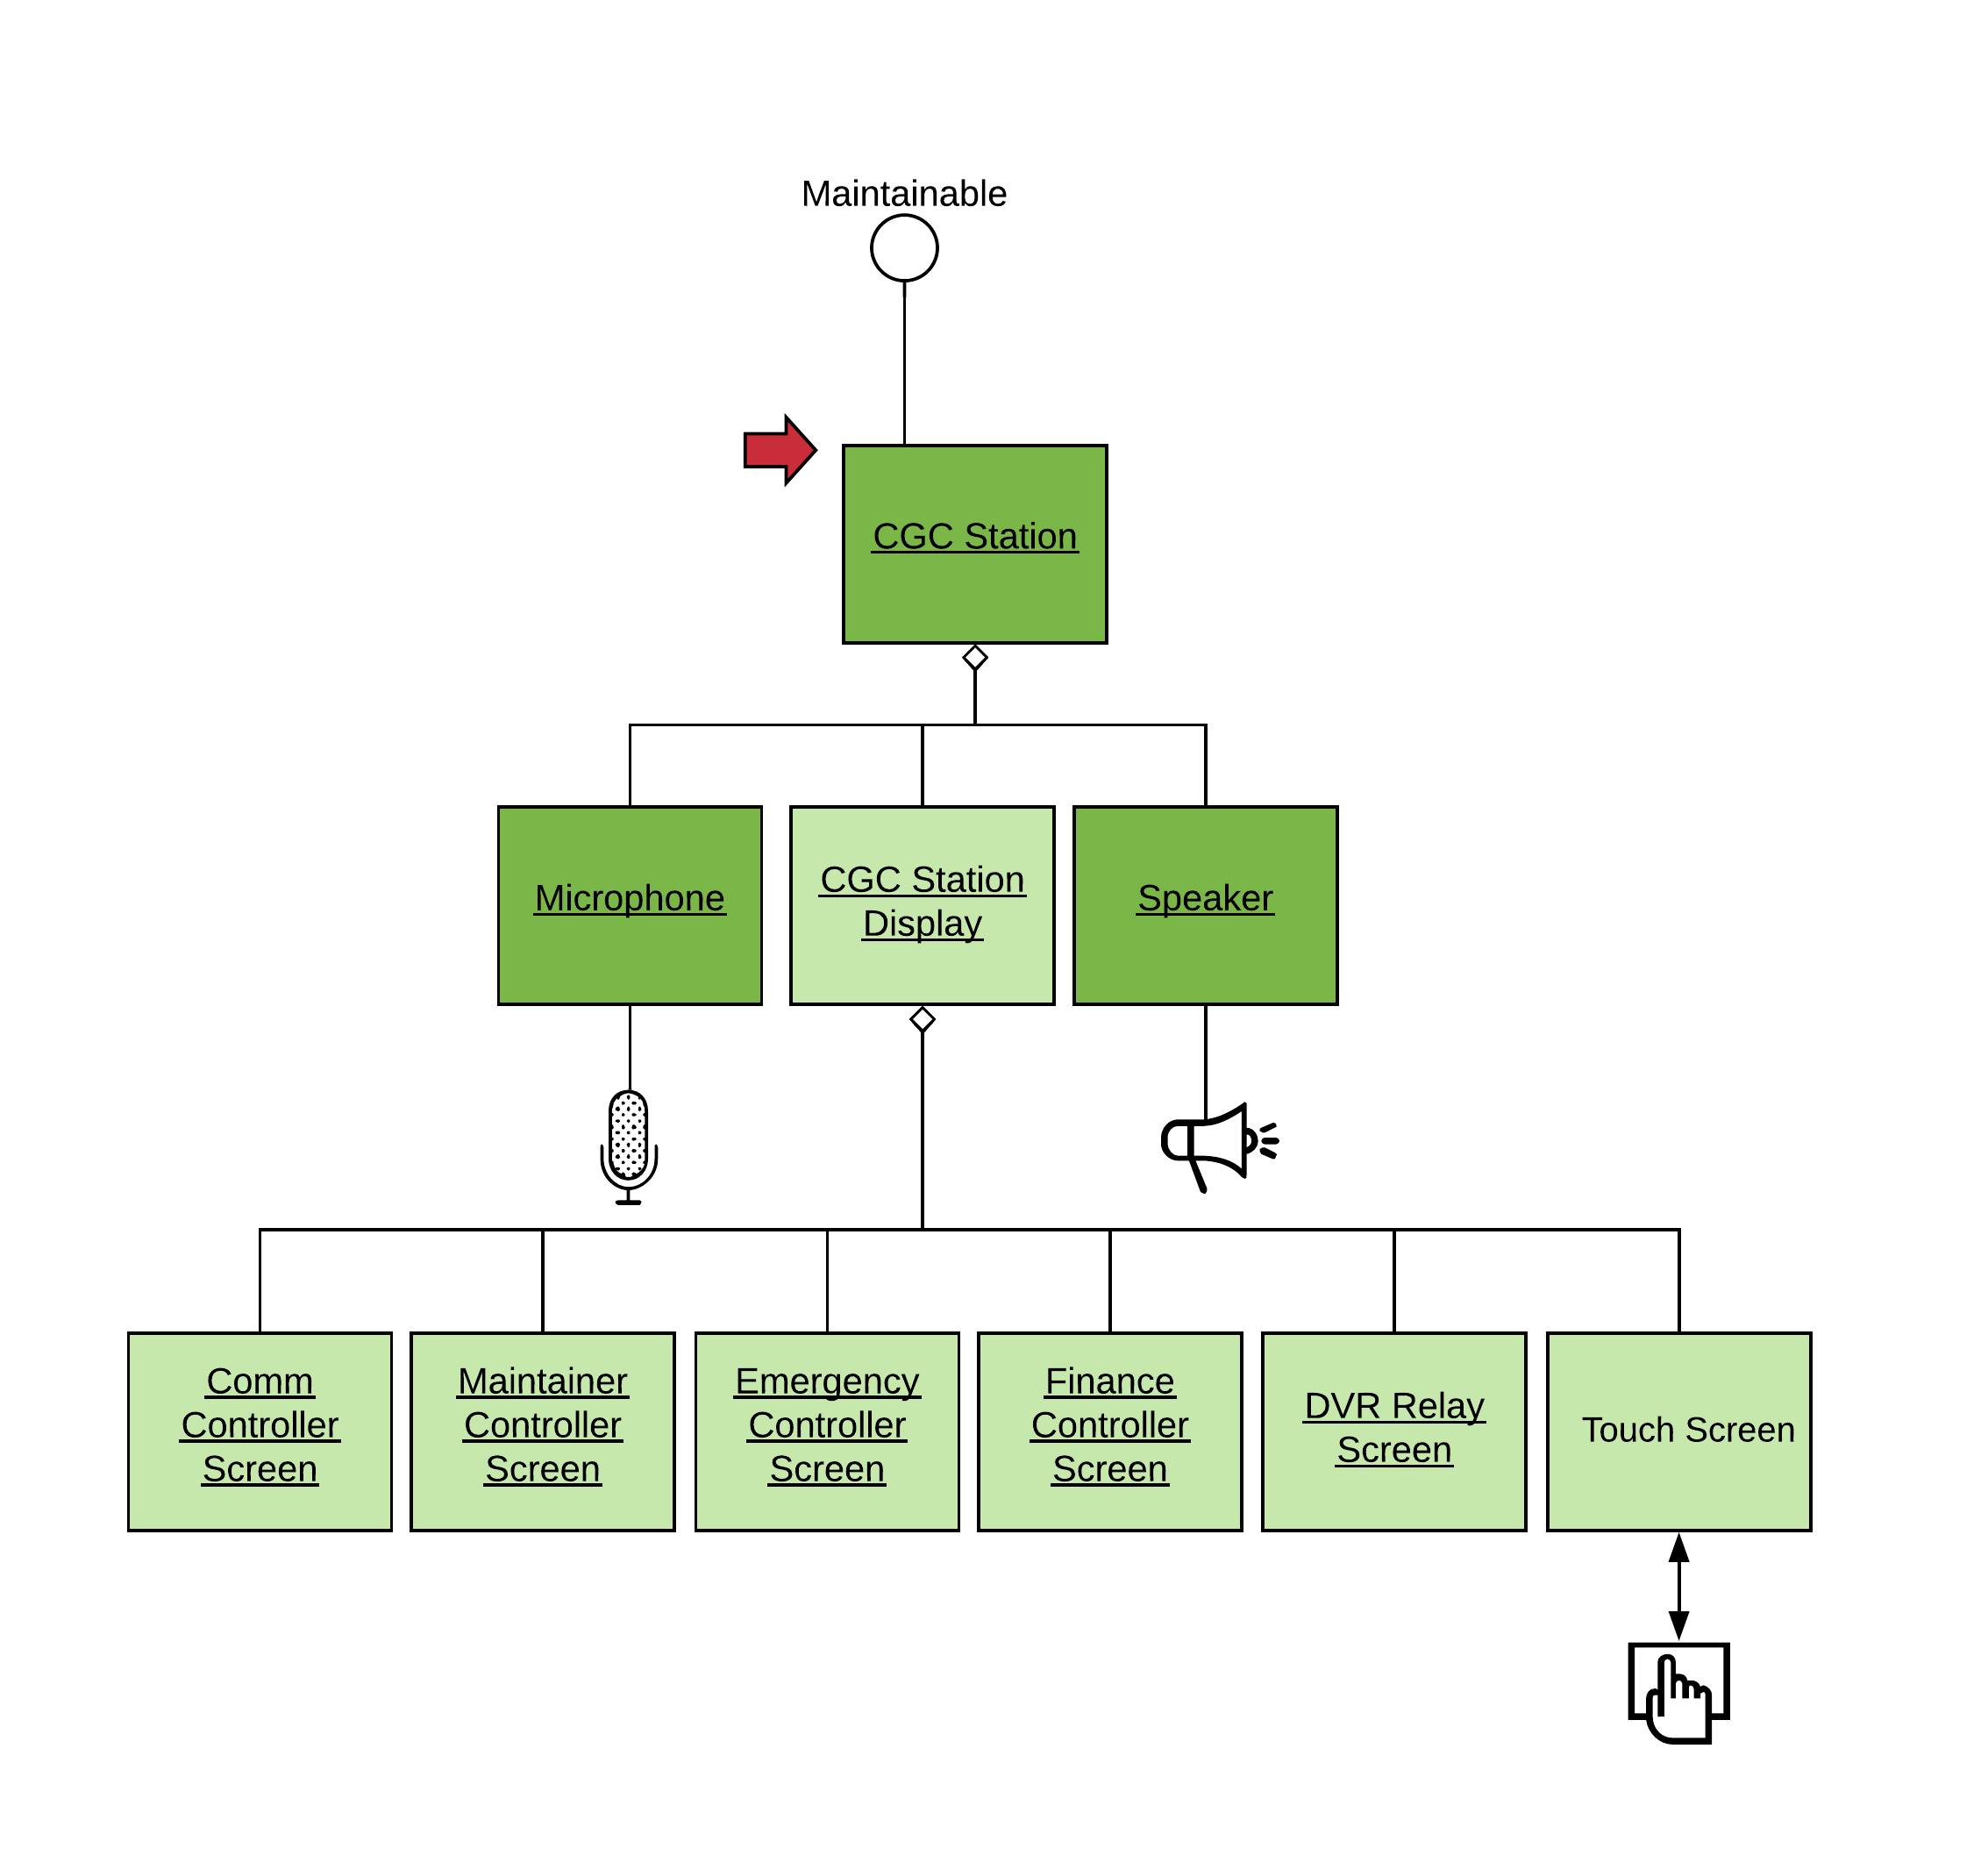
\includegraphics[scale=.20]{CGCStation.png}}
    \caption{\textbf{CGC Station: } A critical device that interfaces employees with the CGC System. we 
clearly see that the device interfaces with a microphone and speaker. these are critical for 
intercom communication to and from other devices. There is also a touch display with a user interface 
that helps the Employee  obtain information such as financial information, the health status of all 
devices, and other screens. It is a device that itself is Maintainable and also reports it's health.}
    \label{fig:CGCStation}
\end{figure}
  

\begin{figure}[H]
    \centerline{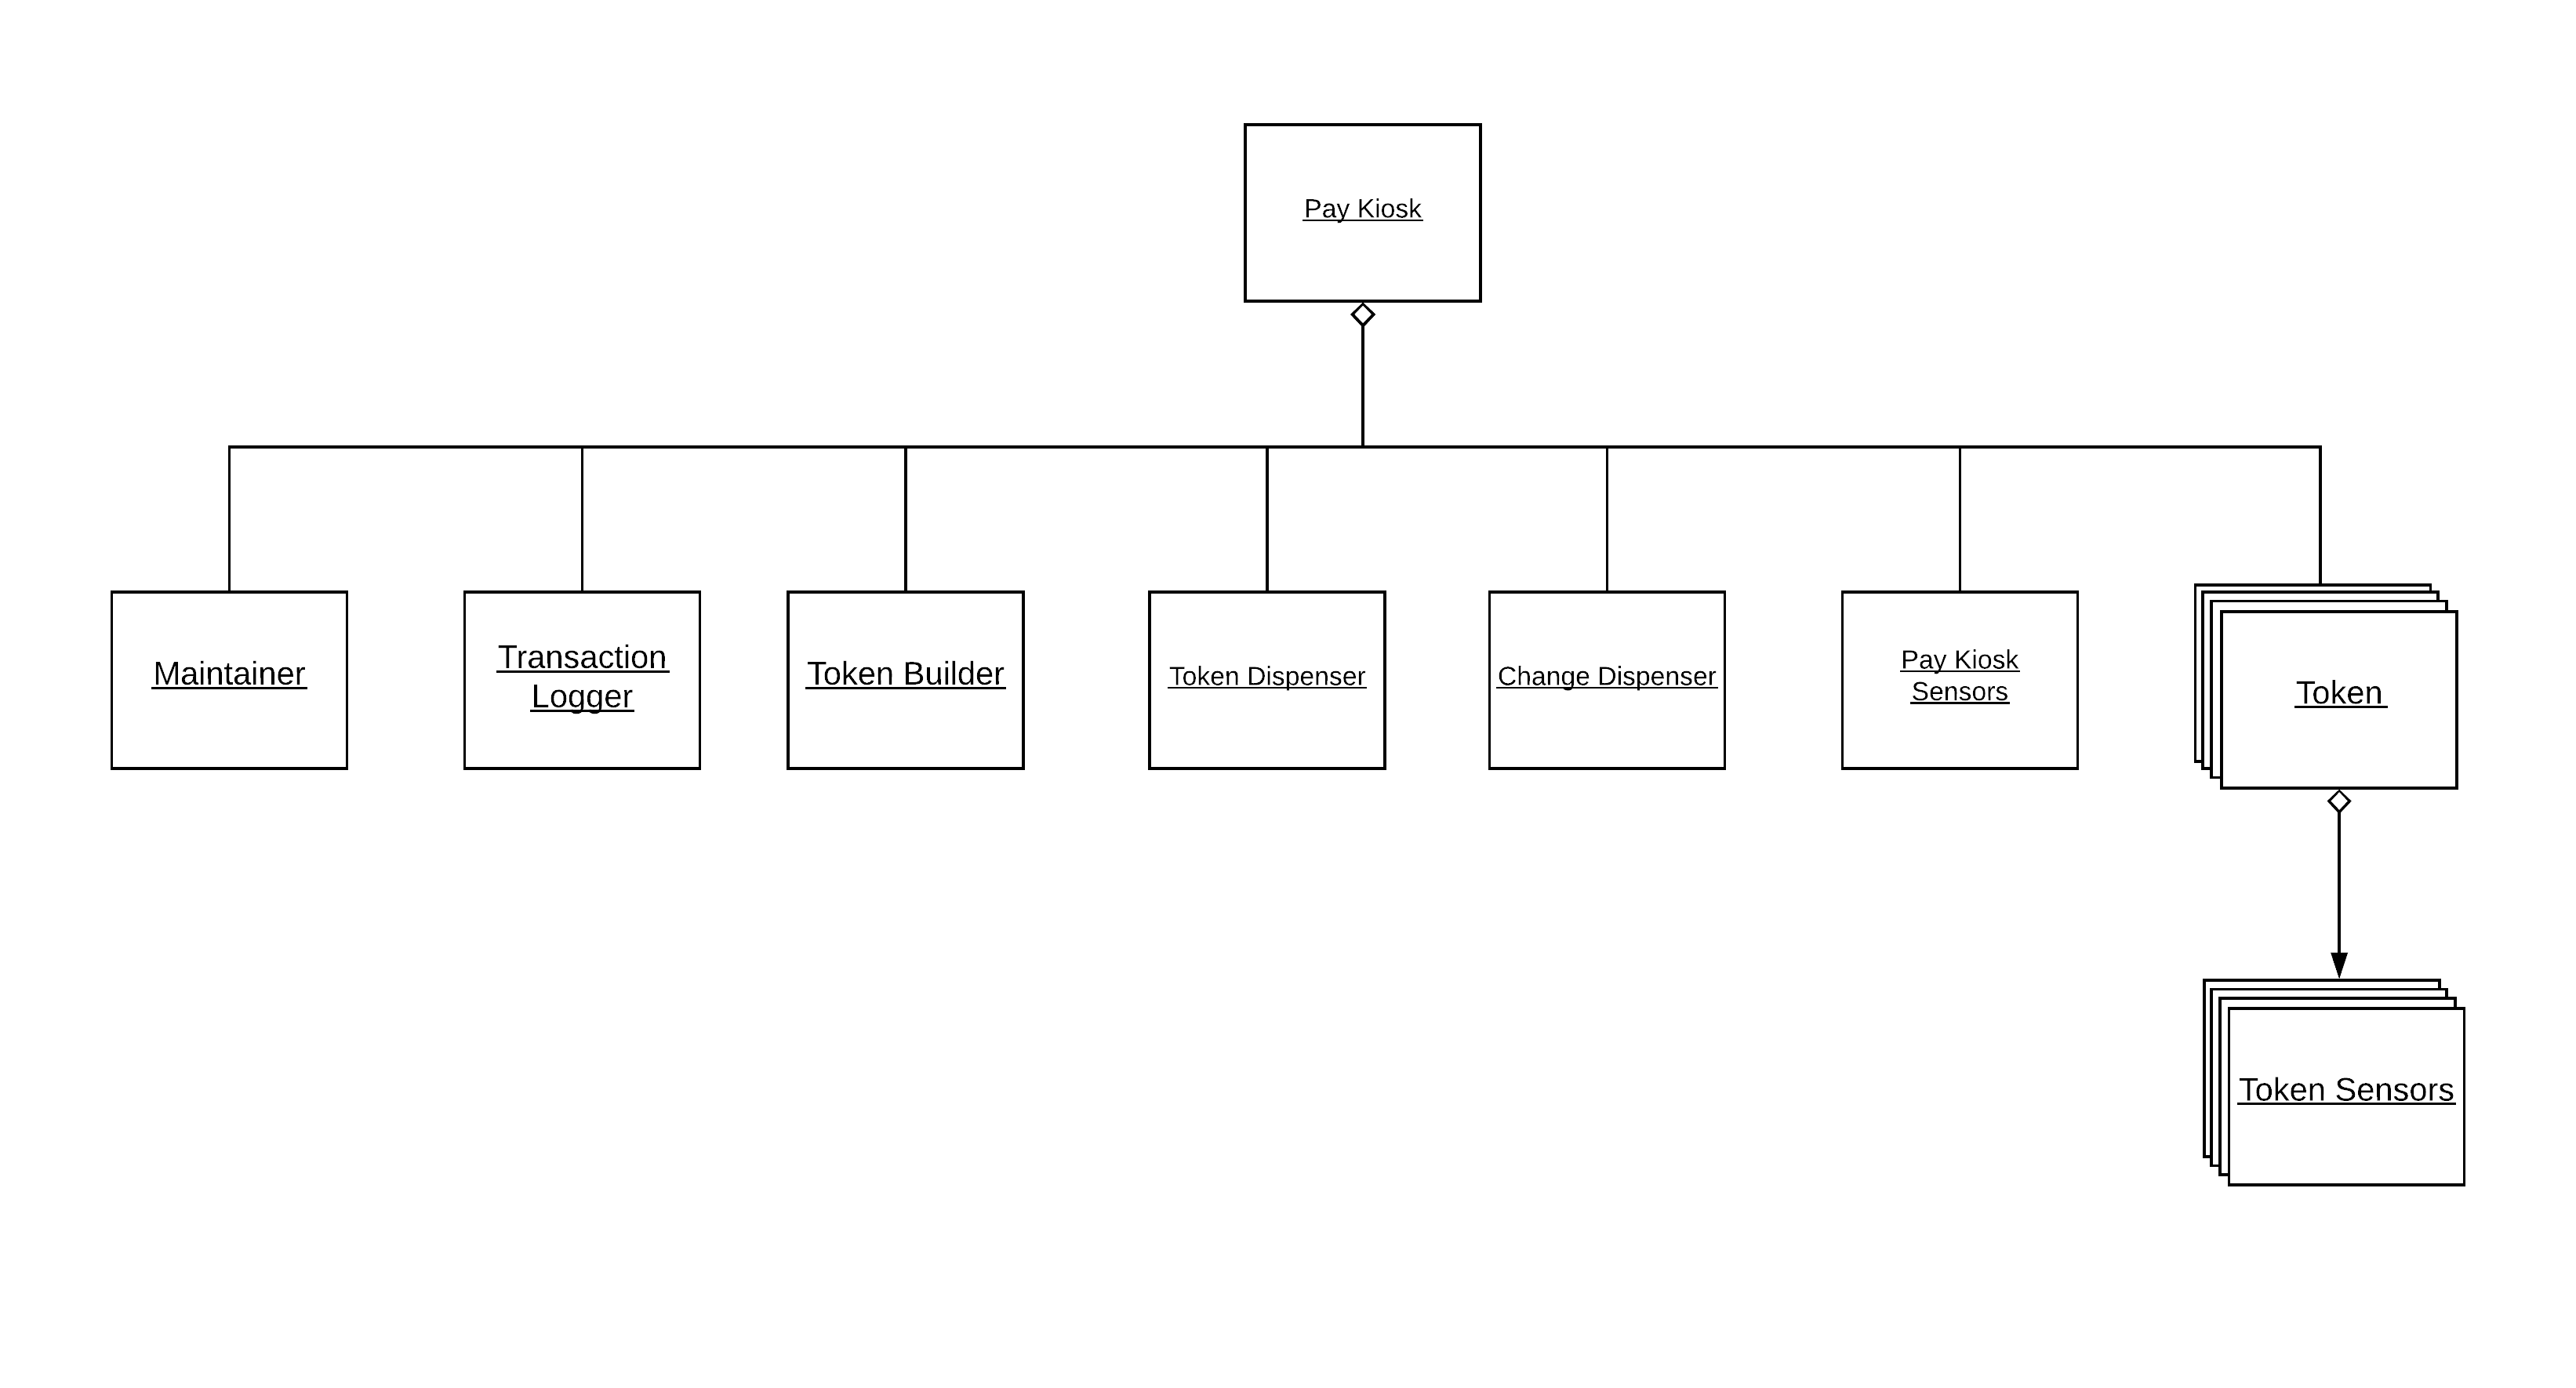
\includegraphics[scale=.20]{PayKiosk.png}}
    \caption{\textbf{The Pay Kiosk: }The Pay Kiosk object controls the Pay Kiosk device. These are devices used to 
purchase and build access Tokens for the visitors. It is critical as it helps the users get into 
the Gardens while also helping the client make money. It is composed of objects that are hardware such
 as the token and change dispensors. it also contains other sensors such as credit card and cash 
 recepticles as well as a touch screen. It has a system that helps log transactions and build tokens. 
 It will configure another critical device, the Token. this is a high tech piece of equipment that is 
 used by the visitor as an access card, but also a communication device, a gps device, as well as 
 other interactive capabilities.}
    \label{fig:PayKiosk}
\end{figure} 


\begin{figure}[H]
    \centerline{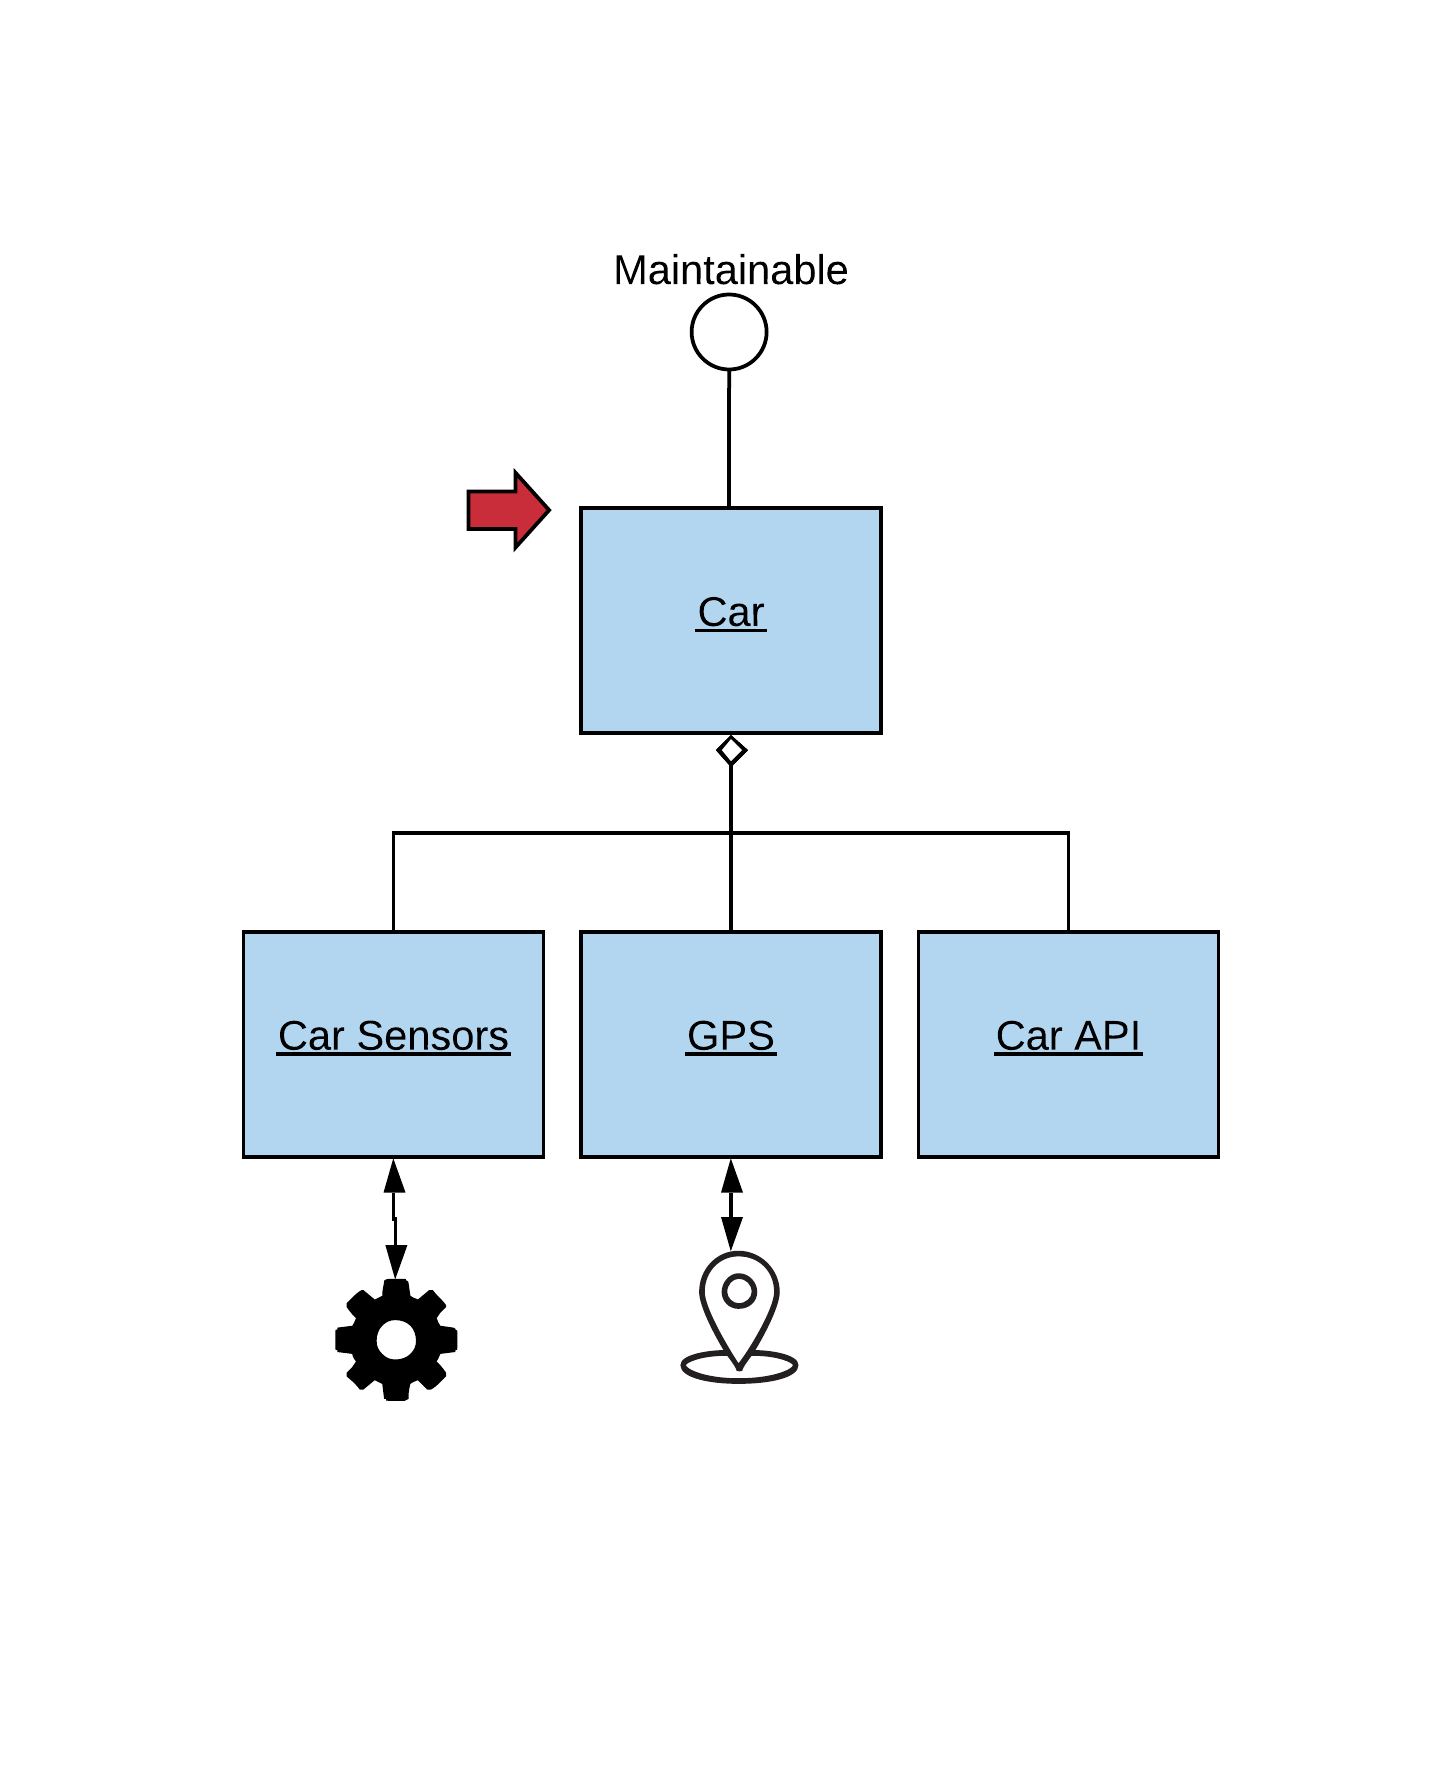
\includegraphics[scale=.20]{Car.png}}
    \caption{\textbf{The Car: }The car object is another critical device. it is a layer on top of the contracted car 
manufacture's own software layer for their autonomous vehicle. It can communicate with sensors such as 
weight sensors, seatbelt sensors, and much more. It has a GPS that communicates with the GPS Server. 
It also includes API's that can be used to give it a destination, override the controls and other such 
capabilitites. It is also a Maintainable object.}
    \label{fig:Car}
\end{figure}

\begin{figure}[H]
    \centerline{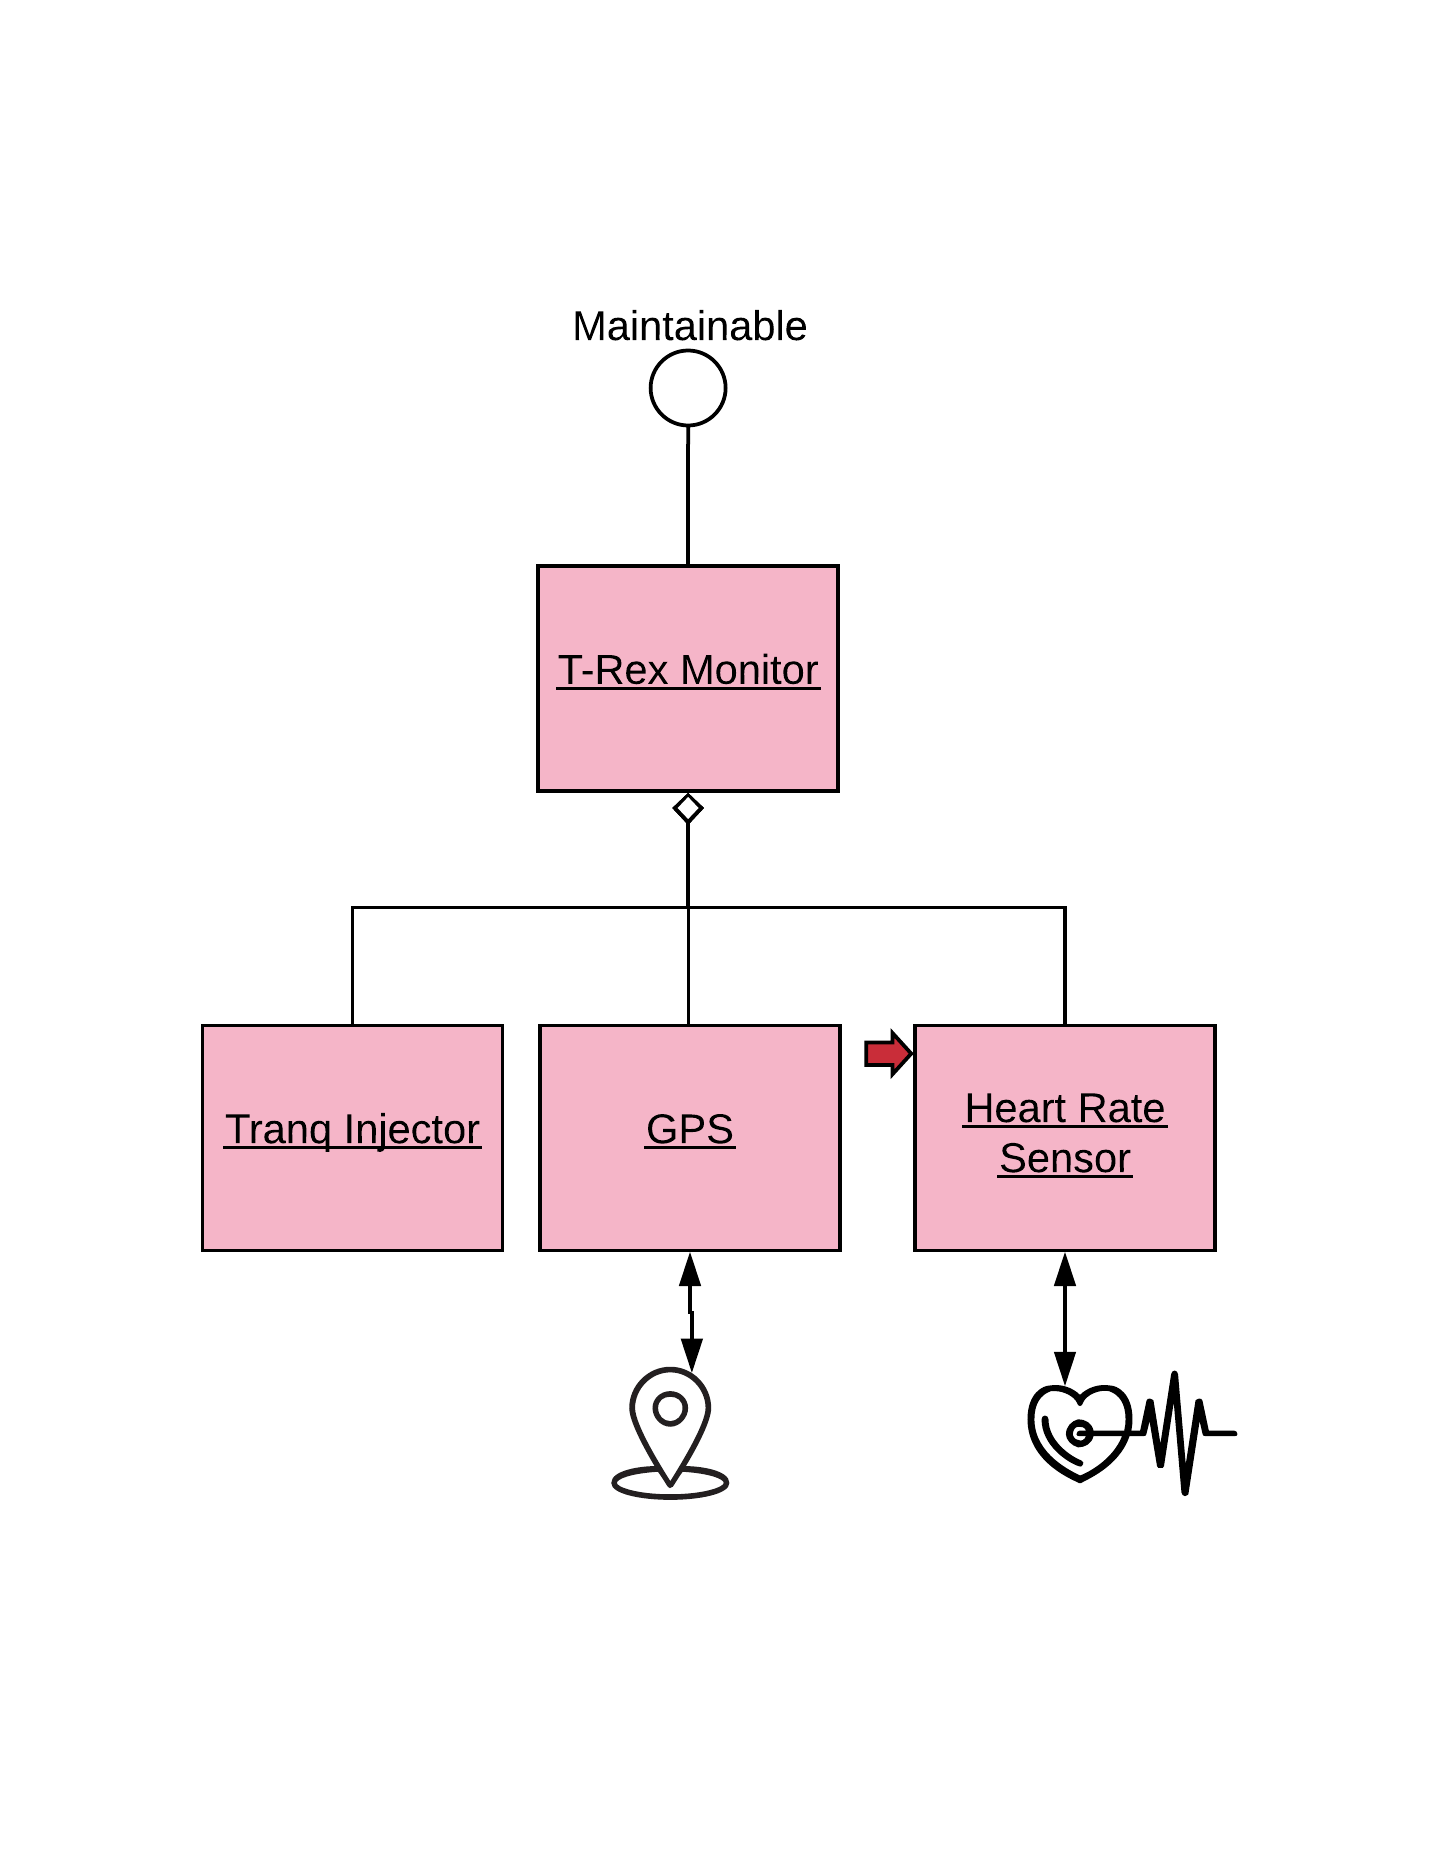
\includegraphics[scale=.20]{TRexMonitor.png}}
    \caption{\textbf{The T-Rex Monitor: }The T-Rex Monitor  helps the CGC keep track of the T-Rex. 
It monitors it's Biometrics to make sure it is not stressed out. it also controls a tranquilizor 
that can put the dino to sleep in a safe mannor. This is another Maintainable system. }
    \label{fig:TRexMonitor}
\end{figure}

\begin{figure}[H]
    \centerline{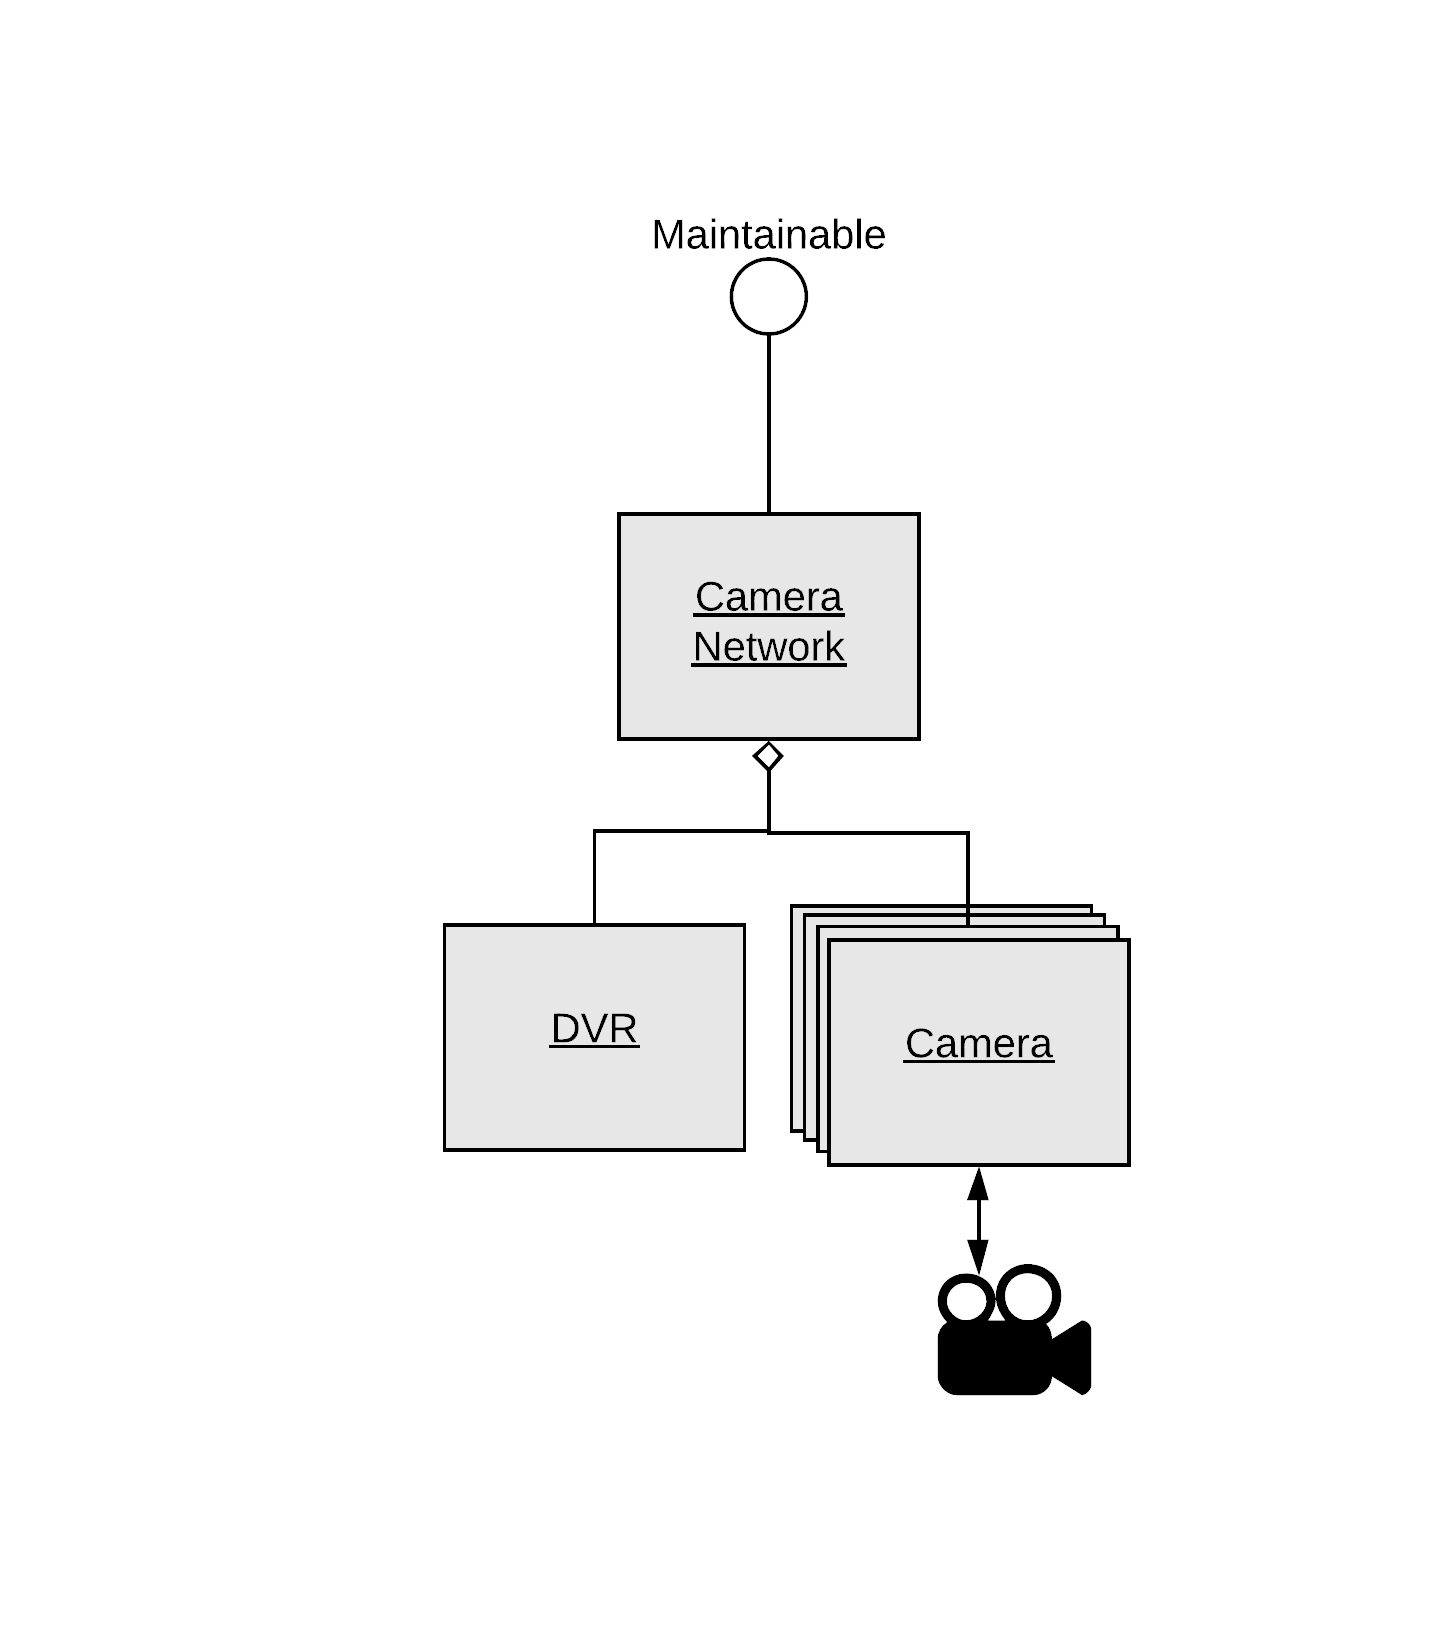
\includegraphics[scale=.20]{CameraNetwork.png}}
    \caption{\textbf{The Camera Network: }The Camera Network Object has one goal and that is to control every single Camera feed. 
It connects this camera feed to a DVR system to help record the feed. It is a Maintainable system.}
    \label{fig:CameraNetwork}
\end{figure}    

\begin{figure}[H]
    \centerline{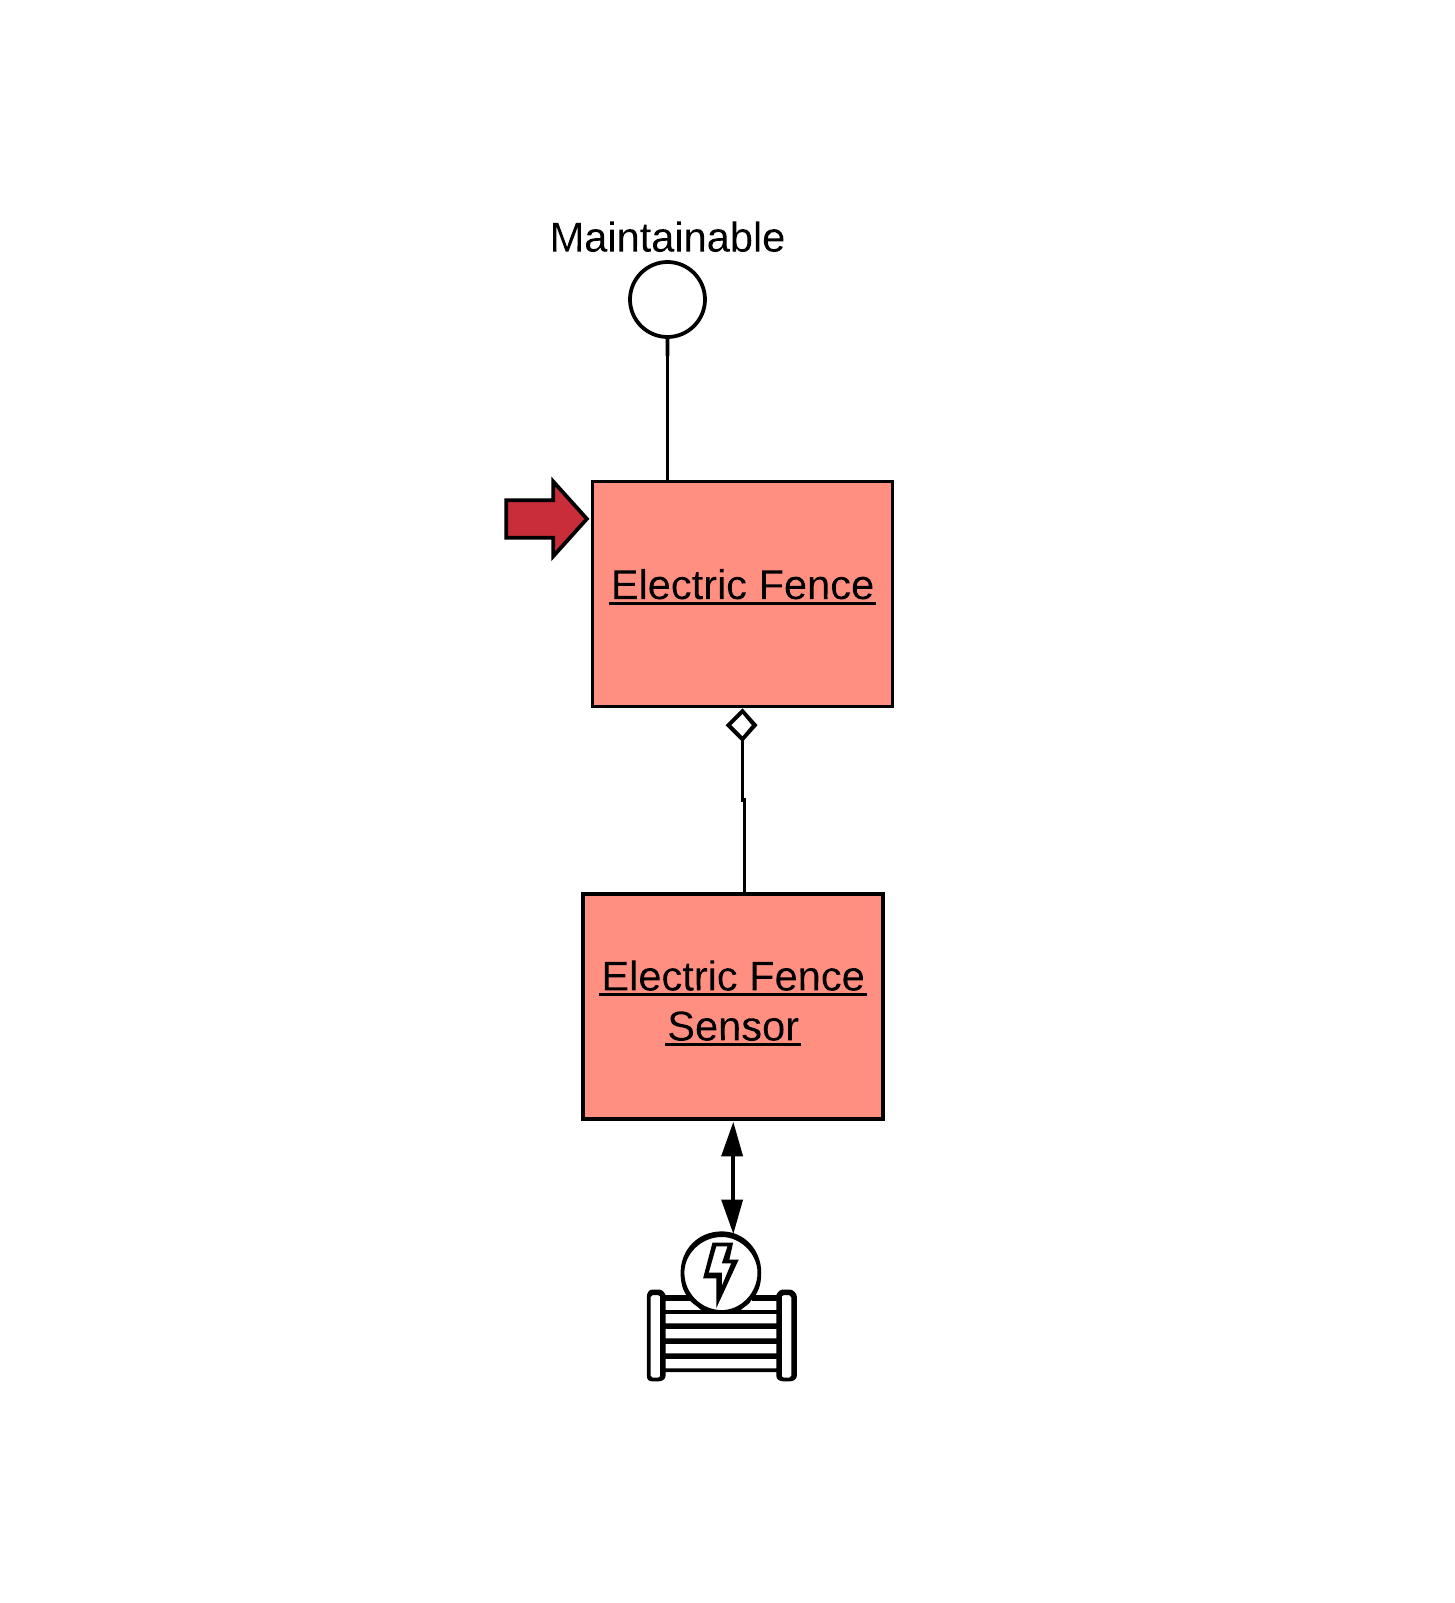
\includegraphics[scale=.20]{ElectricFence.png}}
    \caption{\textbf{The Electric Fence: }The is another very simple software system. The entire goal is to monitor the 
electric fence. To do this it utilizes the Electric Fence Sensor. It is also Maintainable.}
    \label{fig:ElectricFence}
\end{figure}   


\begin{figure}[H]
    \centerline{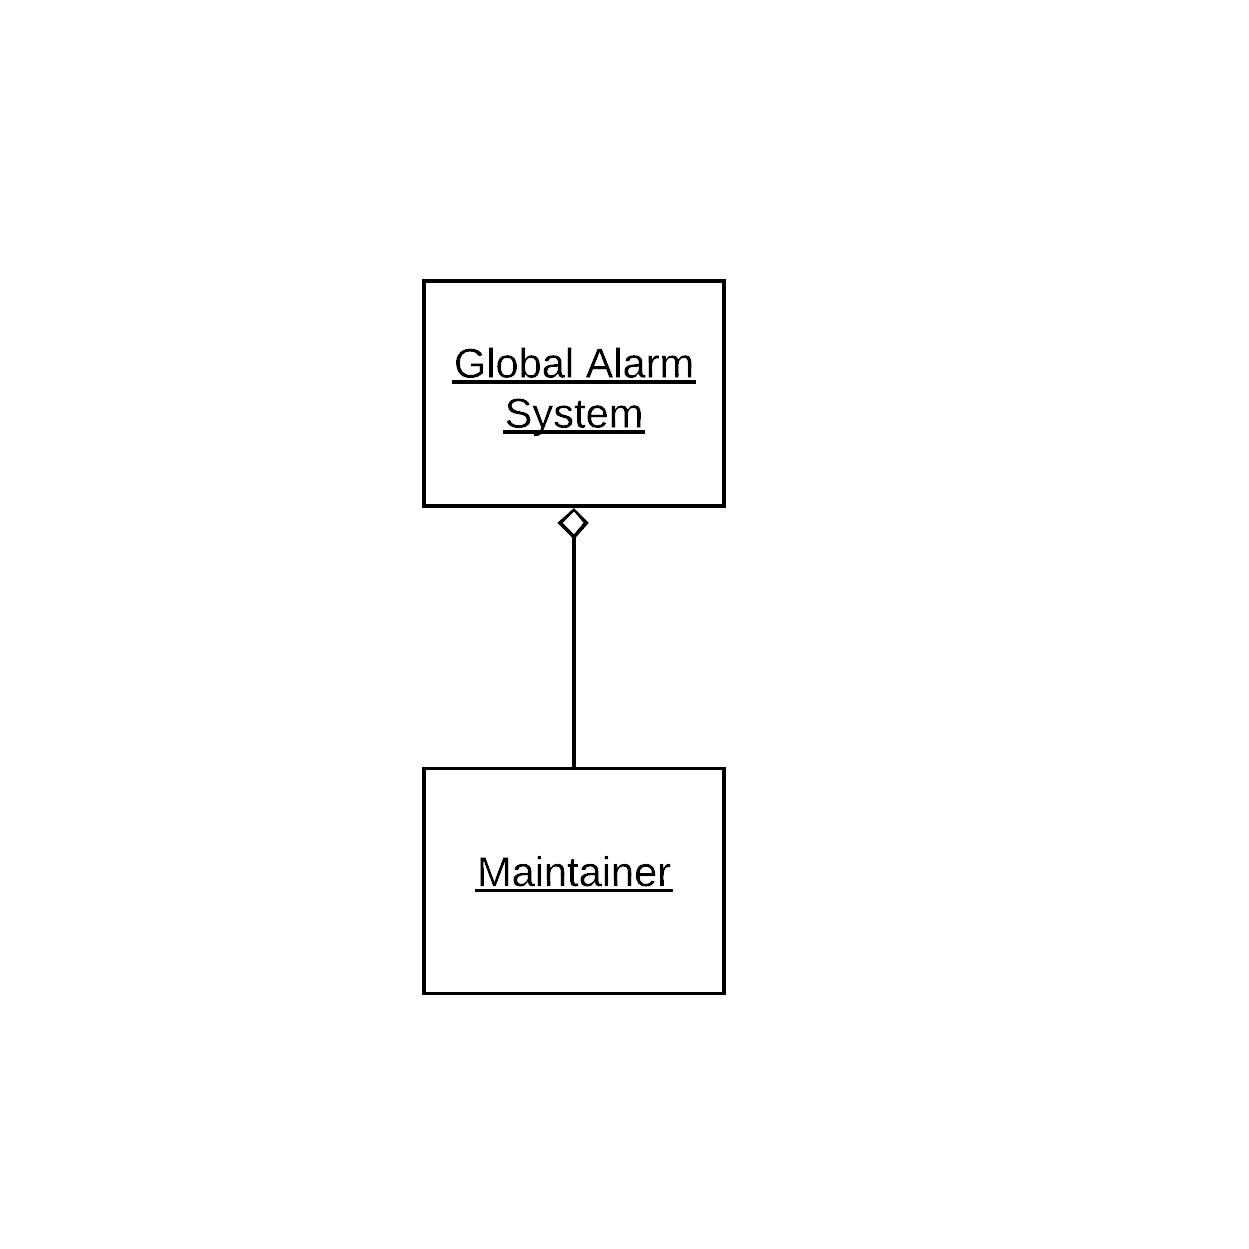
\includegraphics[scale=.20]{GlobalAlarm.png}}
    \caption{\textbf{The Global Alarm System: }The global alarm system controls the loud PA speakers on the island and is critical
 in case of an emergency. This will be able to report on its health by implementing the maintainable 
 interface. It is very basic and the CGC can broker connections to it from CGC Stations.}
    \label{fig:GlobalAlarm}
\end{figure}  

\begin{figure}[H]
    \centerline{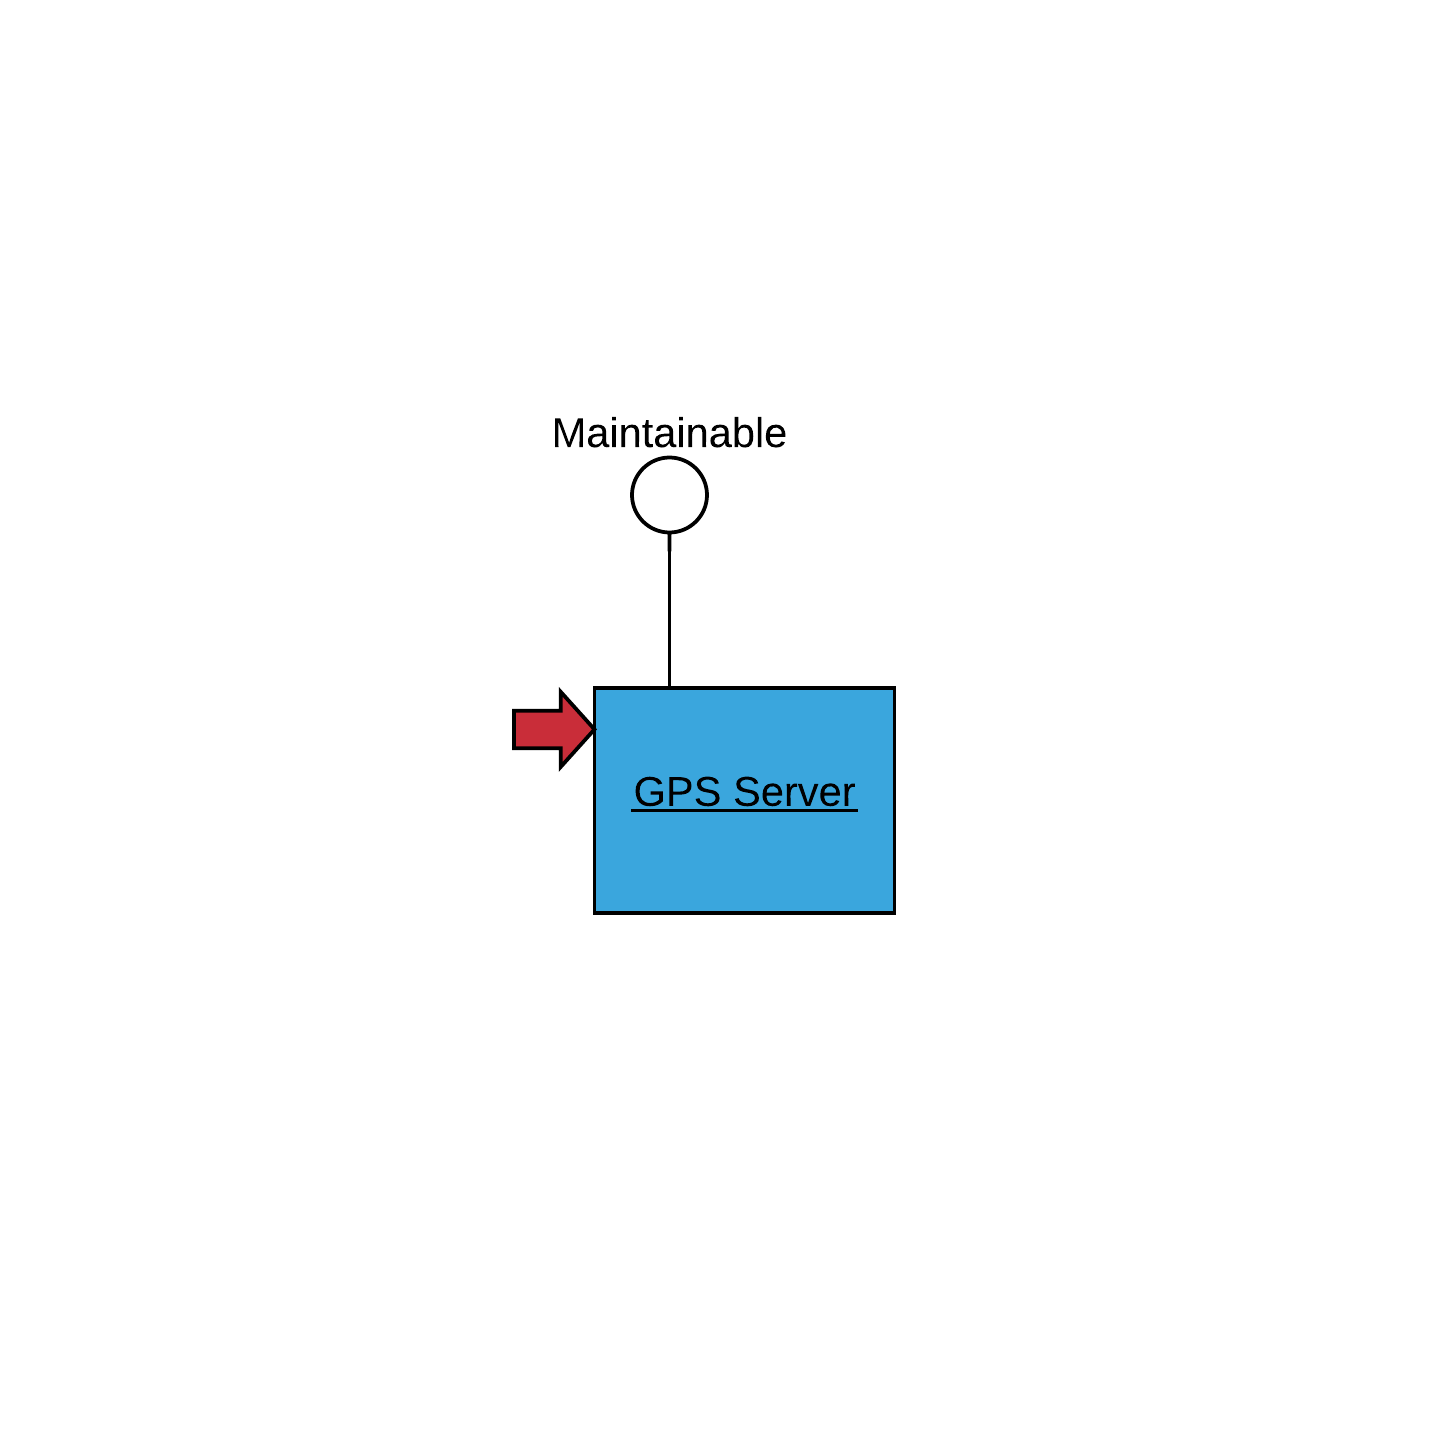
\includegraphics[scale=.20]{GPSServer.png}}
    \caption{\textbf{The GPS Server: }The GPS server is a central server that keeps track of all Registered and active GPS devices. 
It contians the locations of all devices and these are made available through functions. the server will be able 
to report its health by implementing the maintianable interface.}
    \label{fig:GPSServer}
\end{figure}   

\section{Component Specifications} \label{specs}
\paragraph{} \textit{Here are the class specifications\footnote{Component specifications by Anas and Siri.} for objects 
found in Section \ref{over}. The most important attributes and functions are given and where appropriate, any expected 
preconditions, parameters, return values, and post conditions are included. Explanations are given for each component, but 
it should be noted that helper functions are not shown, as they are entrusted with the programmer. Important fields and helper
fields are treated analogously.}

\begin{table}[H]
\begin{tabularx}{\hsize}{|Y|Y|}
    \hline
    \rowcolor{nicegreen}
    \multicolumn{2}{|c|}{\textbf{CGC Class }} \\
    \hline
    \hline
    \multicolumn{2}{|c|}{\textbf{Attributes}}      \\
    \hline
    \textbf{RegisteredTokens} & keeps track of registered visitors to the park. \\
    \textbf{ActiveStation} & checks to ensure CGC stations are active. \\
    \textbf{ActivePayKiosks} & checks to ensure Pay Kiosks are active.  \\
    \textbf{ActiveCars} &  keeps track of active cars. \\
    \textbf{InactiveCars} & keeps tracks of inactive cars. \\
    \hline
    \multicolumn{2}{|c|}{\textbf{Functions}} \\
    \hline
    \textbf{logTransaction(transanction)} & $\rightarrow$ will write the transaction to the finance controller. \\
    \textbf{queryFinanceState(SQLScript)} & $\rightarrow$ return the query results. \\
    \textbf{queryHealthState(SQLScript)} & $\rightarrow$ return the query results. \\
    \textbf{getAllGPSLocations()} & $\rightarrow$ forward all gps locations from the GPS Server. \\
    \textbf{registerToken(tokenID) } & $\rightarrow$ activate token. \\
    \textbf{retireToken(tokenID)} & $\rightarrow$  removes the token from the registered list and cleanly shuts down necessary tasks.\\
    \textbf{relayVideoStream(cameraID, stationID)} & $\rightarrow$ bridge video stream to station. \\
    \textbf{triggerEmergencyMode()} & $\rightarrow$ goes to emergency mode.\\
    \textbf{deactivateEmergencyMode()} & $\rightarrow$ goes back to normal mode operations.\\
    \textbf{activateCar()} & $\rightarrow$  this will activate a new car from the parking lot. \\
    \textbf{bridgeIntercom(carID, stationID)} & $\rightarrow$ this will start a communication link and return null if a fialure.\\
    \textbf{brokerGAConn(stationID)} & $\rightarrow$ returns false for global alarm connection if already in use. \\
    \hline

\end{tabularx}
\end{table}

\begin{table}[H]
\begin{tabularx}{\hsize}{|Y|Y|}
    \hline
    \rowcolor{nicegreen}
    \multicolumn{2}{|c|}{\textbf{Maintainer Class*}} \\ 
    \hline
    \hline
    \multicolumn{2}{|c|}{\textbf{Attributes}}      \\
    \hline
    \textbf{health status} & indicates the health of the appropriate sub-component system. \\
    \hline
    \multicolumn{2}{|c|}{\textbf{Functions}} \\
    \hline
    \textbf{systemCheck()} & $\rightarrow$ performs checks on the system. \\
    \textbf{maintainanceMode()} & $\rightarrow$ goes into maintainance mode. \\
    \hline

\end{tabularx}
     * : {In order to be not repetitive in the sub-components, this class is shown once here and 
is representative of all the sub-components it belongs to.} \\
\end{table}


\begin{table}[H]
\begin{tabularx}{\hsize}{|Y|Y|}
    \hline
    \rowcolor{nicegreen}
    \multicolumn{2}{|c|}{\textbf{Electric Fence Class}} \\ 
    \hline
    \hline
    \multicolumn{2}{|c|}{\textbf{Attributes}}      \\
    \hline
    \textbf{currentMode} & indicates whether or not which mode is detected. \\
    \textbf{Electric Fence Sensor} &  object that senses any distortions in the fence.\\
    \textbf{Maintainer} &  object that checks for health status of the fence.\\
    \hline
    \multicolumn{2}{|c|}{\textbf{Functions}} \\
    \hline
    \textbf{checkStatus()} & $\rightarrow$ checks the status of the fence. \\
    \textbf{switchMode(mode)} & $\rightarrow$ switches the mode based on the specification by CGC. \\
    \textbf{reportHealthToCGC()} & $\rightarrow$ reports the health of the fence. \\
    \hline

\end{tabularx}
\end{table}


\begin{table}[H]
\begin{tabularx}{\hsize}{|Y|Y|}
    \hline
    \rowcolor{nicegreen}
    \multicolumn{2}{|c|}{\textbf{Electric Fence Sensor Class}} \\ 
    \hline
    \hline
    \multicolumn{2}{|c|}{\textbf{Attributes}}      \\
    \hline
    \textbf{electric conductance} & senses electricity in the fence. \\
    \hline
    \multicolumn{2}{|c|}{\textbf{Functions}} \\
    \hline
    \textbf{checkElectricConductance()} & $\rightarrow$ check possible distortions in thefence. \\
    \hline

\end{tabularx}
\end{table}

\begin{table}[H]
\begin{tabularx}{\hsize}{|Y|Y|}
    \hline
    \rowcolor{nicegreen}
    \multicolumn{2}{|c|}{\textbf{Camera Network Class}} \\ 
    \hline
    \hline
    \multicolumn{2}{|c|}{\textbf{Attributes}}      \\
    \hline
    \textbf{Camera} & software that is responsible for streaming video. \\
    \textbf{DVR} &  software that is responsible for storing/retain video.\\
    \textbf{Maintainer} &  object that checks for health status of the fence.\\
    \hline
    \multicolumn{2}{|c|}{\textbf{Functions}} \\
    \hline
    \textbf{checkCameraStatus(cameraID)} & $\rightarrow$ checks the status of the camera. \\
    \textbf{deleteRecording(cameraID, date range)} & $\rightarrow$ delete the recording from a given camera from specified range. \\
    \textbf{activateRecording(cameraID)} & $\rightarrow$ begin recording the given camera. \\
    \textbf{monitor(cameraID)} & $\rightarrow$ view the associated camera. \\
    \textbf{reportOutage()} & $\rightarrow$ report for any possible camera outage upon CGC request. \\
    \hline

\end{tabularx}
\end{table}

\begin{table}[H]
\begin{tabularx}{\hsize}{|Y|Y|}
    \hline
    \rowcolor{nicegreen}
    \multicolumn{2}{|c|}{\textbf{Camera Class}} \\ 
    \hline
    \hline
    \multicolumn{2}{|c|}{\textbf{Attributes}}      \\
    \hline
    \textbf{cameraID} & The camera number. \\
    \textbf{status} & The camera status. \\
    \hline
    \multicolumn{2}{|c|}{\textbf{Functions}} \\
    \hline
    \textbf{getID()} & $\rightarrow$ gives the id of the camera. \\
    \textbf{play()} & $\rightarrow$ starts streaming the video. \\
    \textbf{getStatus()} & $\rightarrow$ gives the status of the camera. \\
    \textbf{getStream()} & $\rightarrow$ view camera. \\
    \hline

\end{tabularx}
\end{table}

\begin{table}[H]
\begin{tabularx}{\hsize}{|Y|Y|}
    \hline
    \rowcolor{nicegreen}
    \multicolumn{2}{|c|}{\textbf{DVR Class}} \\ 
    \hline
    \hline
    \multicolumn{2}{|c|}{\textbf{Attributes}}      \\
    \hline
    \textbf{streamRecord} & keeps track of video streams. \\
    \hline
    \multicolumn{2}{|c|}{\textbf{Functions}} \\
    \hline
    \textbf{start(cameraID)} & $\rightarrow$ begin recording of the camera. \\
    \textbf{delete(cameraID, range)} & $\rightarrow$ delete video stream. \\
    \hline

\end{tabularx}
\end{table}

\begin{table}[H]
\begin{tabularx}{\hsize}{|Y|Y|}
    \hline
    \rowcolor{nicegreen}
    \multicolumn{2}{|c|}{\textbf{GPS Server Class }} \\
    \hline
    \hline
    \multicolumn{2}{|c|}{\textbf{Attributes}}      \\
    \hline
    \textbf{registeredGPSDevices} & indicates all the valid registered gps devices. \\
    \hline
    \multicolumn{2}{|c|}{\textbf{Functions}} \\
    \hline
    \textbf{pingAll()} & $\rightarrow$ will return true if every registeredDevice responds. \\
    \textbf{ping(gpsID)} & $\rightarrow$ will ping specific GPS node and return true if it responds. \\
    \textbf{getLocation(gpsID)} & $\rightarrow$ will return location. \\
    \textbf{getAllLocations()} & $\rightarrow$  gives list of all gps devices. \\
    \hline

\end{tabularx}
\end{table}

\begin{table}[H]
\begin{tabularx}{\hsize}{|Y|Y|}
    \hline
    \rowcolor{nicegreen}
    \multicolumn{2}{|c|}{\textbf{Global Alarm System Class }} \\
    \hline
    \hline
    \multicolumn{2}{|c|}{\textbf{Attributes}}      \\
    \hline
    \textbf{} &  \\
    \hline
    \multicolumn{2}{|c|}{\textbf{Functions}} \\
    \hline
    \textbf{playEmergencyAlarmSound()} & $\rightarrow$ plays the predevined emergency protocal sounds and message. \\
    \textbf{playMessage(soundStream)} & $\rightarrow$ will transform the  incoming sound stream out to the loud speakers. \\
    \hline

\end{tabularx}
\end{table}


\begin{table}[H]
\begin{tabularx}{\hsize}{|Y|Y|}
    \hline
    \rowcolor{nicegreen}
    \multicolumn{2}{|c|}{\textbf{CGC Station Class }} \\
    \hline
    \hline
    \multicolumn{2}{|c|}{\textbf{Attributes}}      \\
    \hline
    \textbf{currentScreen} & the active screen. \\
    \textbf{intercom} & the intercom to talk any relevant components. \\
    \hline
    \multicolumn{2}{|c|}{\textbf{Functions}} \\
    \hline
    \textbf{startIntercom()} & $\rightarrow$ activate intercom to speak to any specific component. \\
    \textbf{syncEmergencyState(sqlScript)} & $\rightarrow$ queries for the state of emergency. \\
    \textbf{syncHealthState(sqlScript)} & $\rightarrow$ sync the status of all the components. \\
    \textbf{syncFinanceState(sqlScript)} & $\rightarrow$ queries finance and expenses information. \\
    \textbf{activateTranqulizer()} & $\rightarrow$ activates tranquilizer in emergency state.\\
    \hline

\end{tabularx}
\end{table}

checkHealth()
reportBiometricsAlarm()
syncLocation()
InjectDino()

\begin{table}[H]
\begin{tabularx}{\hsize}{|Y|Y|}
    \hline
    \rowcolor{nicegreen}
    \multicolumn{2}{|c|}{\textbf{T-Rex Monitor Class }} \\
    \hline
    \hline
    \multicolumn{2}{|c|}{\textbf{Attributes}}      \\
    \hline
    \textbf{Tranquilizer} & the injection used in emergency state. \\
    \textbf{GPS} & to track location of the T-Rex. \\
    \textbf{Heart Rate Sensor} & to monitor health of the T-Rex. \\
    \hline
    \multicolumn{2}{|c|}{\textbf{Functions}} \\
    \hline
    \textbf{checkHealth()} & $\rightarrow$ checks the heart rate and health of the T-Rex. \\
    \textbf{reportBiometricsAlarm()} & $\rightarrow$ reports behavior of the T-Rex. \\
    \textbf{syncLocation()} & $\rightarrow$ gives the location of the T-Rex. \\
    \textbf{injectDino()} & $\rightarrow$ inject tranquilizer in the emergency state. \\
    \hline

\end{tabularx}
\end{table}


\begin{table}[H]
\begin{tabularx}{\hsize}{|Y|Y|}
    \hline
    \rowcolor{nicegreen}
    \multicolumn{2}{|c|}{\textbf{Pay Kiosk Class }} \\
    \hline
    \hline
    \multicolumn{2}{|c|}{\textbf{Attributes}}      \\
    \hline
    \textbf{Token} & The token for the visitor to get all perks of the park.  \\
    \textbf{TransactionID} & the id of the transaction. \\
    \textbf{MoneyType} & type of money requested upon registration. \\
    \hline
    \multicolumn{2}{|c|}{\textbf{Functions}} \\
    \hline
    \textbf{buildToken()} & $\rightarrow$  builds token and logs transaction.\\
    \textbf{displayPurchaseForm()} & $\rightarrow$ displays the registration form. \\
    \textbf{register(demographics)} & $\rightarrow$ registers the visitor based on the provided information. \\
    \textbf{requestMoney()} & $\rightarrow$ requests for money.\\
    \textbf{acceptMoney(moneyType)} & $\rightarrow$ accepts the appropriate money type. \\
    \textbf{dispense(money, receipt())} & $\rightarrow$ dispenses money with receipt. \\
    \textbf{activateToken(tokenID)} & $\rightarrow$ activates token. \\
    \textbf{dispenseToken(tokenID} & $\rightarrow$ dispenses token. \\
    \hline

\end{tabularx}
\end{table}

\begin{table}[H]
\begin{tabularx}{\hsize}{|Y|Y|}
    \hline
    \rowcolor{nicegreen}
    \multicolumn{2}{|c|}{\textbf{Car Cass }} \\
    \hline
    \hline
    \multicolumn{2}{|c|}{\textbf{Attributes}}      \\
    \hline
    \textbf{isActivated} & Specifies if the car is activated \\
    \textbf{isParked} & Specifies if the car is parked \\
    \textbf{Position} & Specifies where is the car located \\
    \textbf{Destiny} & Destiny where the car has to travel\\
    \textbf{Passengers} & Number of passengers in the car\\
    \hline
    \multicolumn{2}{|c|}{\textbf{Functions}} \\
    \hline
    \textbf{checkPosition()} & $\rightarrow$ Return the position of the car in the island \\
    \textbf{checkIfParked()} & $\rightarrow$ Return if the car is parked \\
    \textbf{isActivated()} & $\rightarrow$ Return if the car is activated \\
    \textbf{activateCar()} & $\rightarrow$ Will activate the car \\
	\textbf{desactivateCar()} & $\rightarrow$ Will desactivate the car  \\
	\textbf{travelToDestiny()} & $\rightarrow$ Will start the trip to the destiny \\
    \textbf{setDestiny()} & $\rightarrow$ Will set the destiny of the car\\
	\textbf{ValidateToken()} & $\rightarrow$ Check if the token is valid \\
	\textbf{lockDoors()} & $\rightarrow$ Will lock the doors of the car \\
	\textbf{unlockDoors()} & $\rightarrow$ Will unlock the doors of the car \\
	\textbf{passengerSit()} & $\rightarrow$ Will recognize that there is a passenger sit and has his belt on \\
	\textbf{sendLocationToCGC()} & $\rightarrow$ Will send the location to GCG \\
    \hline

\end{tabularx}
\end{table}

\section{Sample Use Cases} \label{samp}
\paragraph{} \textit{A broad overview of use cases begins this section and it is followed 
by detailed case descriptions. Human actors are denoted by small stick figures and have the 
same color scheme as the box that contains their labels. The section later features use case 
diagrams for each actor and a detailed sample of use cases.}
%\begin{figure}[H]
%    \centerline{\includegraphics[scale=.30]{ECSUseCaseUML.png}}
%    \caption{Shows the a general view of use cases as a diagram. The primary actors are color coded on the left, and exclusive
%    goals share the same color scheme. Secondary actors are shown on the right. Goals that may be had by various actors have a 
%    grey color scheme. The dashed lines indicate inclusions.}
%    \label{fig:usecasediagram}
%\end{figure}
section{Sample Use Cases}
\paragraph{} \textit{The CGC lends itself for a substantial amount of uses. Some notable uses include financial,
official, managerial, medical, and technical connotations.}

    \subsection{CGC Station Operator}
    \textit{The CGC Station Operator  (GSO)is the actor responsible for monitoring the central CGC system that
    controls all other components. This individual may communicate with guests or other employees 
    through the car intercom, may place vehicles into manual mode, and has access to the camera network.}
    \par\noindent\rule{\textwidth}{0.4pt}    
    \begin{itemize}
        \item[]\textbf{Use Case:}                                
            ReprimandTroublesomeGuest

        \item[]\textbf{Primary Actor:}
            CGC Station Operator

        \item[]\textbf{Goal in Context:}
            To reprimand a guest that is causing trouble by incremental warnings ranging from
            casual notice, to threats of banishment from the resort.

        \item[]\textbf{Preconditions:}
            The system and all components are functioning properly.

        \item[]\textbf{Trigger:}
            A guest is caught throwing rocks into the enclosure.
            
        \item[]\textbf{Scenario:}
            \begin{enumerate}
                \item The GSO reviews an alert from the electric fence interface.
                \item The GSO reads that small voltage spikes have been detected.
                \item The GSO heads to the surveillance camera that corresponds to the
                panel in question.
                \item The GSO observes a guest hurling rocks at the enclosure, which
                explains the voltage spikes.
                \item The GSO immediately and firmly tells the guest to stop throwing rocks
                through the PA system near the site.
                \item The GSO is ignored by the guest who gives the finger to the camera.
                \item The GSO dispatches the nearest patrol vehicle to the location.
                \item The GSO explains the situation to the security guard that happens 
                to be in the patrol vehicle at the time.
                \item The GSO firmly alerts the unruly guest that a security guard has been sent.
                \item The security guard arrives and reprimands the guest.
                \item The guest become violent and gets tased and pepper sprayed.
                \item The guest is apprehended and placed in the patrol vehicle.
                \item The GSO dismisses the electric fence alerts.
            \end{enumerate}

        \item[]\textbf{Exceptions:}
            \begin{itemize}
                \item[] The system is triggered into emergency mode.
            \end{itemize}

        \item[]\textbf{Priority:}
            Moderate, not necessary, but can be useful.
            
        \item[]\textbf{When Available:}
            On demand.

        \item[]\textbf{Frequency of Use:}
            More frequent with higher volumes of visits.
            
        \item[]\textbf{Channel to Primary Actor:}
            Electric fence panel, CGC Station GUI, camera 

        \item[]\textbf{Secondary Actors:}
            Patrol Vehicle, Security Guard, Electric Fence, Guest
            
        \item[]\textbf{Channels to Secondary Actors:}
            \begin{itemize}
                \item[] Patrol Vehicle: direct
                \item[] Security Guard: car intercom
                \item[] Electric Fence: direct
                \item[] Guest: PA system, electric fence
            \end{itemize}

        \item[]\textbf{Open Issues:}
            \begin{itemize}
                \item[] None known.
            \end{itemize}
    \end{itemize}
     
    \subsection{Emergency Personnel}
    \textit{Emergency Personnel (EP) may be police officers, federal agents, paramedics, and in certain contexts even 
    security guards. Among the many actions that may be taken by such an actor are search and rescue, arrest, perform CPR, 
    and many more.}
    \par\noindent\rule{\textwidth}{0.4pt}    
    \begin{itemize}
        \item[]\textbf{Use Case:}                                
            SearchAndRescue

        \item[]\textbf{Primary Actor:}
            Emergency Personnel

        \item[]\textbf{Goal in Context:}
            To find any potentially remaining guests after a disaster has occurred on the island.
            
        \item[]\textbf{Preconditions:}
            Emergency mode may or may not be currently active, but it has definitely been triggered prior to 
            the arrival of the actor.

        \item[]\textbf{Trigger:}
            A distress signal has been received from Cretaceous Gardens (from Isla Trueno).

        \item[]\textbf{Scenario:}
            \begin{enumerate}
                \item The platoon has received orders to address an emergency on Isla Trueno. 
                \item The troops arrive to the island littered with debris and corpses. 
                \item Some Pay kiosks remain active with an eerie glow coming from an uncannily 
                cheerful welcome screen.
                \item Screams of terror can be heard in the distance, followed by tremendous roars.
                \item The Emergency Personnel head to the kiosks and enter special codes that provide
                them with an enormous supply of token devices.
                \item The EP diffuse throughout the island as they sweep for survivors.
                \item Several helicopters can be heard swarming overhead and small group
                is sent to the CGC Station.
                \item As the troops move inland they find severely injured, but alive, guests.
                \item The troops give the injured new tokens which may be detected by the team
                at the station.
                \item A second group arrives at the island, and is directed by the team at the station
                (via walkie talkies) to the injured.
                \item The team notices the T-Rex Monitor signal moving toward the sweeping group of soldiers
                and they alert them immediately to get into offensive positions.
                \item The helicopters overhead lower themselves to wait for the animal.
                \item Permission to engage is granted and the beast is taken down.
                \item The troops continue their operation until sunrise as teams of paramedics
                are shipped to the island.
            \end{enumerate}

        \item[]\textbf{Exceptions:}
            \begin{itemize}
                \item[] The T.Rex destroys the CGC Station.
            \end{itemize}

        \item[]\textbf{Priority:}
            Essential, must be implemented.
            
        \item[]\textbf{When Available:}
            On demand.

        \item[]\textbf{Frequency of Use:}
            Hopefully never.

        \item[]\textbf{Channel to Primary Actor:}
            Token GPS

        \item[]\textbf{Secondary Actors:}
            Guests, Tokens, Pay Kiosks

        \item[]\textbf{Channels to Secondary Actors:}
            \begin{itemize}
                \item[] Guests: tokens
                \item[] Tokens: pay kiosks
                \item[] Pay Kiosks: direct
            \end{itemize}

        \item[]\textbf{Open Issues:}
            \begin{itemize}
                \item[] None known.
            \end{itemize}
    \end{itemize}
        
    \subsection{Guest}
    \textit{The guest is the primary benefactor of many to the system's features. The primary role of this
    actor is to safely indulge in what the resort has to offer. The most common use for a guest is to see the main
    exhibit but there may be several prerequisite uses that lead up to that.}
    \par\noindent\rule{\textwidth}{0.4pt}    
    \begin{itemize}
        \item[]\textbf{Use Case:}                                
            ViewTRex

        \item[]\textbf{Primary Actor:}
            Guest

        \item[]\textbf{Goal in Context:}
            To see a live dinosaur.

        \item[]\textbf{Preconditions:}
            The system and all components are functioning normally.
            
        \item[]\textbf{Trigger:}
            The guest wishes to see a dinosaur since the age of five.

        \item[]\textbf{Scenario:}
            \begin{enumerate}
                \item Upon hearing of the grand opening of Cretaceous Gardens, the guest immediately
                heads to the island by whatever means possible.
                \item On arrival, the guest witnesses tremendous lines formed at many pay kiosks
                near the entrance of the resort.
                \item After what seems like an eternity, the it is the guest's turn to purchase entry to the resort.
                \item The guest is welcomed through a pleasant graphical display.
                \item The guest is asked a series of questions in order verify compliance with the park policies
                (e.g. How old are you? Do you consent to having your picture taken? Do you accept full responsibility 
                for any injuries sustained due to personal choices? Do you accept the risks of seeing a live 
                Tyrannosaurus Rex and free Cretaceous Gardens of any and all consequences of doing so?)
                \item After ignoring all the fine print and zipping through the legal stuff, the guest finally
                arrives at the screen that will allow the rental of an access token.
                \item The guest enters the amount of time he or she plans to stay and is given the total price.
                \item The guest is prompted to enter payment.
                \item The guest pays after confirmation and receives the rental token device.
                \item Instructions on what to do next are displayed on the kiosk screen.
                \item The guest uses the token device to enter the resort via a small gate.
                \item The guest eventually arrives at a parked car, into which others may or may not be entering.
                \item The guest enters the token device into the seatbelt buckle and secures the seatbelt.
                \item The guest lets the car do its job (see section \ref{carscenarios}).
                \item The guest arrives at the exhibit and exits the car, taking the token device along.
                \item The guest heads toward another gate which scans the token device to provide access.
                \item The guest sprints toward the enclosure.
                \item The guest is lucky and gets to see the mighty T.Rex sniffing around. 
            \end{enumerate}

        \item[]\textbf{Exceptions:}
            \begin{itemize}
                \item[] Guest changes his or her mind anywhere in the scenario and decides to leave.
                \item[] The system is triggered into emergency mode.
            \end{itemize}

        \item[]\textbf{Priority:}
            Essential, must be implemented.

        \item[]\textbf{When Available:}
            On Demand.

        \item[]\textbf{Frequency of Use:}
            Up to thousands of times per day.

        \item[]\textbf{Channel to Primary Actor:}
            Direct.

        \item[]\textbf{Channels to Secondary Actors:}
            *means through which the primary and secondary actors interact*
            \begin{itemize}
                \item[] Kiosk: Display on kiosk.
                \item[] Token: Device desplay and speaker.
                \item[] Guest Vehicle: Token interrfaces and seat sensors.
                \item[] T-Rex: Seen through enclosure fence.
            \end{itemize}
        \item[]\textbf{Secondary Actors:}
            Kiosk, Token, Guest Vehicle, T-Rex.

        \item[]\textbf{Open Issues:}
            None known.
    \end{itemize}

    \par\noindent\rule{\textwidth}{0.4pt}    
    \begin{itemize}
        \item[]\textbf{Use Case:}                                
            Evacuate

        \item[]\textbf{Primary Actor:}
            Guest

        \item[]\textbf{Goal in Context:}
            To leave the island as quickly and as safely as possible.

        \item[]\textbf{Preconditions:}
            There exists some imminent threat to the guest (it may be an enclosure failure, inclement 
            weather, or any other emergency of similar caliber). Sudden guest death (unrelated to the
            island or system) may also be the case.

        \item[]\textbf{Trigger:}
            Something horrible occurs. For simplicity, the following scenario assumes the T-Rex destroys
            its enclosure and is now on the loose.

        \item[]\textbf{Scenario:}
            \begin{enumerate}
                \item The T-Rex destroys the enclosure (see subsection \ref{trexleave}).
                \item Emergency mode is activated.
                \item22 All guests are alerted via the car intercom, the token devices, and an
                island wide speaker system, the Global Alarm System.
                \item Guests receive instructions via the above means with interleaved reassurances
                that extra vehicles are on the way to pick them up.
                \item Guests are also informed that they may enter any vehicle, with or without tokens.
                \item Once in the vehicle, guests are asked (via the token device) whether or not
                they would like to depart.
                \item If at least one individual submits a yes, the car transmits a message to indicate
                imminent departure with a warning that doors will soon close.
                \item Once in motion, the guest in the driver seat is offered the option to place the vehicle into
                manual mode.
                \item If the individual chooses to do so, then he or she may now pilot the vehicle as he or she wishes.
                \item Otherwise, the car will head south as quickly and as safely as possible.
                \item Once at the south end, the car will park and wait for guests to exit.
                \item After it has been confirmed that no guests remain in the vehicle (seat weight sensors
                indicate all seats are empty), the guests are given another warning to stand back.
                \item As the guests head toward the exit, the car closes its doors and speeds north 
                to collect more guests.
            \end{enumerate}

        \item[]\textbf{Exceptions:}
            \begin{itemize}
                \item[] The car suffers damage that causes it to malfunction.
            \end{itemize}

        \item[]\textbf{Priority:}
            Essential, must be implemented.

        \item[]\textbf{When Available:}
            On demand.

        \item[]\textbf{Frequency of Use:}
            Hopefully never, but at least once in reality.

        \item[]\textbf{Channel to Primary Actor:}
            Car doors, tokens, interior car components (if manual mode is enabled)
            
        \item[]\textbf{Channels to Secondary Actors:}
            \begin{itemize}
                \item[] T-Rex: breached enclosure
                \item[] Token: device display and speaker
                \item[] Emergency Personnel: directly at any stage during the evacuation.
            \end{itemize}
        \item[]\textbf{Secondary Actors:}
            T.Rex, Tokens, Emergency Personnel

        \item[]\textbf{Open Issues:}
            \begin{itemize}
                \item[] None known.
            \end{itemize}
    \end{itemize}
    
    % another use case
    
    % another use case
    
    % ...
    
    \subsection{Guest Vehicle}\label{carscenarios}
    \textit{The guest vehicle (GV) plays a vital role in facilitating the guest experience. The actor primarily
    moves guests to and from the exhibit, but may exhibit other functions when the system is in maintenance or
    emergency mode.}
    \par\noindent\rule{\textwidth}{0.4pt}    
    \begin{itemize}
        \item[]\textbf{Use Case:}                                
            ShuttleGuestsToExhibit

        \item[]\textbf{Primary Actor:}
            Guest Vehicle

        \item[]\textbf{Goal in Context:}
            To transport guests to the northern part of the island so they may 
            visit the exhibit.

        \item[]\textbf{Preconditions:}
            The system is in normal mode and all components are functioning properly.

        \item[]\textbf{Trigger:}
            A transaction is confirmed and a tokens are provided to guests.

        \item[]\textbf{Scenario:}
            \begin{enumerate}
                \item The guests are directed to the parked GV.
                \item The guests enter the GV.
                \item The GV instructs guests to enter their token devices into their belt buckles.
                \item The GV detects all token-containing buckles have been used to fasten corresponding seatbelts.
                \item The GV locks its doors and unlocks window functionality for guests.
                \item The GV performs a quick system check.
                \item The GV heads toward the exhibit.
                \item The GV arrives and parks in front of a gate that leads to the exhibit.
                \item The GV reminds the guests to take their tokens with them as it grants them access through the gate.
                \item The guests exit the vehicle and make their way toward the gate.
                \item The GV parks itself nearby and starts a timer.
            \end{enumerate}

        \item[]\textbf{Exceptions:}
            \begin{itemize}
                \item[] A guest loses his or her token device, thus preventing seatbelt access, which necessitates
                staff intervention.
            \end{itemize}

        \item[]\textbf{Priority:}
            Essential, must be implemented.

        \item[]\textbf{When Available:}
            On Demand.

        \item[]\textbf{Frequency of Use:}
            Up to thousands of times per day.
            
        \item[]\textbf{Channel to Primary Actor:}
            Direct.

        \item[]\textbf{Secondary Actors:}
            Guests, CGC Station Operator, Tokens
            
        \item[]\textbf{Channels to Secondary Actors:}
            \begin{itemize}
                \item[] Guests: doors, seatbelts, speakers
                \item[] CGC Station Operator: direct
                \item[] Tokens: seatbelt buckles
            \end{itemize}

        \item[]\textbf{Open Issues:}
            \begin{itemize}
                \item[] None known.
            \end{itemize}
    \end{itemize}

    \par\noindent\rule{\textwidth}{0.4pt}    
    \begin{itemize}
        \item[]\textbf{Use Case:}                                
            ShuttleGuestsFromExhibit

        \item[]\textbf{Primary Actor:}
            Guest Vehicle

        \item[]\textbf{Goal in Context:}
            To transport guests to the southern part of the island so they may 
            leave the island.

        \item[]\textbf{Preconditions:}
            The system is in normal mode and all components are functioning properly.

        \item[]\textbf{Trigger:}
            The guests' time is up at the exhibit.

        \item[]\textbf{Scenario:}
            \begin{enumerate}
                \item The car alerts the guests it shuttled to the exhibit that time is up.
                \item The guests hear the alert from the car and from their token devices.
                \item Some of the guests immediately head to the car while others delay.
                \item The guests that head to the car enter it and fasten their seat belts.
                \item The GV sends another alert to those remaining.
                \item The rest of the guests finally arrive and enter the GV.
                \item The GV locks its doors after everyone has fastened their seatbelts.
                \item The GV heads south.
                \item The GV arrives to the southern part of the island where it parks.
                \item The guests release their seatbelts.
                \item The GV unlocks its doors and allows the guests to exit.
                \item The GV is dispatched elsewhere.
            \end{enumerate}

        \item[]\textbf{Exceptions:}
            \begin{itemize}
                \item[] A guest happens to be injured and requires another type of transportation.
                \item[] A guest loses his or her token device, thus preventing seatbelt access.
            \end{itemize}

        \item[]\textbf{Priority:}
            Essential, must be implemented.

        \item[]\textbf{When Available:}
            On Demand.

        \item[]\textbf{Frequency of Use:}
            Up to thousands of times per day.
            
        \item[]\textbf{Channel to Primary Actor:}
            Direct.

        \item[]\textbf{Secondary Actors:}
            Guests, CGC Station Operator, Tokens
            
        \item[]\textbf{Channels to Secondary Actors:}
            \begin{itemize}
                \item[] Guests: doors, seatbelts, speakers
                \item[] CGC Station Operator: direct
                \item[] Tokens: seatbelt buckles
            \end{itemize}

        \item[]\textbf{Open Issues:}
            \begin{itemize}
                \item[] None known.
            \end{itemize}
    \end{itemize}
    
    \subsection{Maintenance Personnel}
    \textit{Maintenance Personnel (MP) is responsible for the physical connections 
    and addressing any issues with the physical components used with by the CGC (e.g cameras, 
    kiosks, cars, enclosure panels, etc.). This individual would be in charge of responding to nodal failures.}
    \par\noindent\rule{\textwidth}{0.4pt}    
    \begin{itemize}
        \item[]\textbf{Use Case:}                                
            RepairExternalEnclosureCamera

        \item[]\textbf{Primary Actor:}
            Network Maintenance Personnel

        \item[]\textbf{Goal in Context:}
            To fix or replace a malfunctioning or broken camera that has been detected to
            be in such a state by the CGC. The camera in question resides outside the exhibit
            enclosure.

        \item[]\textbf{Preconditions:}
            The CGC is not in emergency mode but may be in either normal or maintenance mode, and
            the issue has already been diagnosed (i.e. it is known with certainty that the problem
            is the camera and not the link to the camera).

        \item[]\textbf{Trigger:}
            The CGC reports an error in some camera within the Camera Network after 
            failing to make contact via alternate paths.

        \item[]\textbf{Scenario:}
            \begin{enumerate}
                \item NMP is dispatched and transported in an self-driving car to the 
                location of the problem by the CGC Station Operator (CSO).
                \item NMP arrives and performs a repair, exchanges the broken camera
                for a new one, or attaches a new one if it happens to be gone all together.
                \item The CSO and NMP perform tests to ensure proper function.
                \item The maintenance is concluded.
                \item The NMP is dispatched to any other components that may need servicing.
                \item [OR]
                \item The NMP returns any removed parts (e.g. the broken camera) to a stock room.
            \end{enumerate}

        \item[]\textbf{Exceptions:}
            \begin{itemize}
                \item[] Maintenance materials are out of stock.
                \item[] Emergency mode interrupts the procedure.
            \end{itemize}

        \item[]\textbf{Priority:}
            Moderate, should be implemented.

        \item[]\textbf{When Available:}
            On Demand.

        \item[]\textbf{Frequency of Use:}
            It may vary with respect to the average lifetime of the cameras in the network.

        \item[]\textbf{Channel to Primary Actor:}
            CGC Station, Car, Camera, Camera Network

        \item[]\textbf{Secondary Actors:}
            CGC Station Operator, Camera Network
            
        \item[]\textbf{Channels to Secondary Actors:}
            \begin{itemize}
                \item[] CGC Station Operator: Car Intercom
                \item[] Camera Network: Camera
            \end{itemize}

        \item[]\textbf{Open Issues:}
            \begin{itemize}
                \item[] None known
            \end{itemize}
    \end{itemize}
%    
%    % another use case
%    
%    % another use case
%    
%    % ...
    
    \subsection{Patrol Vehicle}
    \textit{This actor is a special type of autonomous vehicle that patrols the island for an 
    added layer of protection and in the interest of guest welfare.}
    \par\noindent\rule{\textwidth}{0.4pt}    
    \begin{itemize}
        \item[]\textbf{Use Case:}                                
            PatrolIsland

        \item[]\textbf{Primary Actor:}
            Patrol Vehicle

        \item[]\textbf{Goal in Context:}
            To provide a means via which security personnel may patrol the island. The vehicles
            are to be on a mostly predetermined route, so the security guards (in this context)
            are mostly passive agents.

        \item[]\textbf{Preconditions:}
            The system is in normal mode and all components are functioning properly.

        \item[]\textbf{Trigger:}
            The resort opens for business.

        \item[]\textbf{Scenario:}
            \begin{enumerate}
                \item Cretaceous Gardens opens to employees before opening for the business day.
                \item The Patrol Vehicle (PV) is dispatched via a routine protocol.
                \item The PV performs a test run around the island before picking up the security guard
                of the shift.
                \item The security guard enters the PV, after which the PV performs another test trip.
                \item The security guard double checks state of the route.
                \item Anything out of the ordinary is reported to the relevant parties (maintenance for example).
                \item The PV returns to the southern part of the island.
                \item The security guard confirms an all clear with other employees.
                \item The rest of the employees continue their setup as the security guard enters the PV.
                \item The PV begins its daily patrolling routine (one or more simple circuits around the island).
            \end{enumerate}

        \item[]\textbf{Exceptions:}
            \begin{itemize}
                \item[] The system is triggered into emergency mode.
            \end{itemize}

        \item[]\textbf{Priority:}
            Low, not necessary but may be useful.

        \item[]\textbf{When Available:}
            During business hours.

        \item[]\textbf{Frequency of Use:}
            Daily.

        \item[]\textbf{Channel to Primary Actor:}
            Direct.

        \item[]\textbf{Secondary Actors:}
            CGC Station Operator, Security Guard
            
        \item[]\textbf{Channels to Secondary Actors:}
            \begin{itemize}
                \item[] Security Guard: Car door, inner components of car 
                \item[] CGC Station Operator: CGC station interface
            \end{itemize}

        \item[]\textbf{Open Issues:}
            \begin{itemize}
                \item[] None known.
            \end{itemize}
    \end{itemize}
%    
%    % another use case
%    
%    % another use case
%    
%    % ...

    \subsection{Sales department}
    \textit{The sales department (SD) is, for the sake of simplicity, is the actor interested 
    in maximizing ticket sales and profits. The SD is interested in any financial trends
    for the sake of such aims. They may also be interested in finding efficiency bottle necks
    that incur unnecessary costs.}
    \par\noindent\rule{\textwidth}{0.4pt}    
    \begin{itemize}
        \item[]\textbf{Use Case:}                                
            VisualizeSalesData

        \item[]\textbf{Primary Actor:}
            Sale Department

        \item[]\textbf{Goal in Context:}
            To acquire and study data related to sales within some given period of time.

        \item[]\textbf{Preconditions:}
            The system is not in emergency mode nor maintenance mode and all components are 
            functioning properly.

        \item[]\textbf{Trigger:}
            It is about time to wrap up a fiscal quarter to plan for the next one.

        \item[]\textbf{Scenario:}
            \begin{enumerate}
                \item A meeting is scheduled in order to plan for the next quarter.
                \item The SD gathers all sales data provided by the CGC.
                \item The SD uses a provided interface to organize the data into meaningful visualizations.
                \item The SD exports the visualizations for a presentation at the meeting.
                \item The meeting is held and the SD presents their findings.
                \item The SD contribution helps guide the conversation for what to do next.
                \item The meeting concludes. 
            \end{enumerate}

        \item[]\textbf{Exceptions:}
            \begin{itemize}
                \item[] The system enter emergency mode.
            \end{itemize}

        \item[]\textbf{Priority:}
            Extremely low, need not be implemented.

        \item[]\textbf{When Available:}
            On demand.

        \item[]\textbf{Frequency of Use:}
            May be used continuously (as a live data feed), or any number of snapshots
            may be taken hourly, daily, weekly, etc.

        \item[]\textbf{Channel to Primary Actor:}
            An auxiliary interface specialized for financial data visualization.

        \item[]\textbf{Secondary Actors:}
            CGC Control Station
            
        \item[]\textbf{Channels to Secondary Actors:}
            \begin{itemize}
                \item[] CGC Control Station: some network link to forward relevant data
            \end{itemize}

        \item[]\textbf{Open Issues:}
            \begin{itemize}
                \item[] An interface separate from the Control Station interface would have to
                be developed as it would reside elsewhere on the island.
            \end{itemize}
    \end{itemize}
    
    % another use case
    
    % another use case
    
    % ...

%%%%% Siri %%%%%
    \subsection{System Administrator}
    \textit{The this actor (SA) specializes in addressing hardware issues with the CGC Station. This
    individual is responsible for repairing disk drives, monitors, redundancy elements within the
    station, updating machine operating systems, etc.}
    \par\noindent\rule{\textwidth}{0.4pt}    
    \begin{itemize}
        \item[]\textbf{Use Case:}                                
            UpgradeSystemMemory

        \item[]\textbf{Primary Actor:}
            CGC System Technician

        \item[]\textbf{Goal in Context:}
            To upgrade the memory of the machines within at CGC Control Station (e.g. add 16 GB RAM).

        \item[]\textbf{Preconditions:}
            The CGC is not in emergency mode but may be in either maintenance or normal mode.

        \item[]\textbf{Trigger:}
            Cretaceous Gardens experiences an increase in demand, which (if the trend continues) will
            require more computational resources to handle more guests, more efficiently.

        \item[]\textbf{Scenario:}
            \begin{enumerate}
                \item The Sales Department notices a distinct upward trend in sales.
                \item The findings percolate through the relevant business entities within the company.
                \item The CST is dispatched to the Control Station.
                \item The CST enables maintenance mode.
                \item The CST upgrades machines that are currently being used for redundancy.
                \item The CST enables maintenance mode on the redundant machines.
                \item The redundant machines and active machines, switch roles.
                \item The CST upgrades the now-redundant machines.
                \item The CST performs tests.
                \item The CST disables maintenance mode in both active, and redundant machines.
            \end{enumerate}

        \item[]\textbf{Exceptions:}
            \begin{itemize}
                \item[] The trend is ignored by management.
            \end{itemize}

        \item[]\textbf{Priority:}
            Moderate, should be implemented.

        \item[]\textbf{When Available:}
            On demand.

        \item[]\textbf{Frequency of Use:}
            Every two or three fiscal years.

        \item[]\textbf{Channel to Primary Actor:}
            Control station hardware.
        
        \item[]\textbf{Secondary Actors:}
            Sales Department, CGC Control Station, Pay Kiosk
                
        \item[]\textbf{Channels to Secondary Actors:}
            \begin{itemize}
                \item[] Sales Department: pay kiosk transaction logs
                \item[] CGC Control Station: direct access
                \item[] Pay Kiosk: direct connection
            \end{itemize}

        \item[]\textbf{Open Issues:}
            \begin{itemize}
                \item[] None known.
            \end{itemize}
    \end{itemize}
    
    \subsection{System Auditor}
    \textit{This actor (SA) may be an external individual that may either be hired by Cretaceous 
    Gardens to test the robustness of the system, or whose inspection may be mandated by law.}
    \par\noindent\rule{\textwidth}{0.4pt}    
    \begin{itemize}
        \item[]\textbf{Use Case:}                                
            SimulateProtocols

        \item[]\textbf{Primary Actor:}
            System Auditor

        \item[]\textbf{Goal in Context:}
            To observe currently implemented protocols within the system and provide an analysis
            regarding their safety.

        \item[]\textbf{Preconditions:}
            The system is not in emergency mode nor maintenance mode, but may be put into such
            modes for testing purposes (presumably outside business hours).

        \item[]\textbf{Trigger:}
            The time for a system audit has arrived, either after being scheduled or at random.

        \item[]\textbf{Scenario:}
            \begin{enumerate}
                \item The SA arrives to the CGC Control Station outside of business hours.
                \item The SA requests to observe a simulation of the currently used functions of the system.
                \item The SA is provided with a set of protocols that may be simulated.
                \item For each protocol, the SA runs a simulation.
                \item The system passes the audit and the SA leaves.
                \item OR
                \item The system fails while simulating one or more protocols and the auditor presents a deadline
                to fix the issue lest a fine is incurred.
            \end{enumerate}

        \item[]\textbf{Exceptions:}
            \begin{itemize}
                \item[] An audit occurs in the middle of a system upgrade.
                \item[] The system is triggered into emergency mode (due to an actual emergency)
            \end{itemize}

        \item[]\textbf{Priority:}
            Low, not explicitly required, but may be useful for legal robustness.

        \item[]\textbf{When Available:}
            On demand.

        \item[]\textbf{Frequency of Use:}
            Annually or less frequently.

        \item[]\textbf{Channel to Primary Actor:}
            CGC Control Station interface

        \item[]\textbf{Secondary Actors:}
            CGC Control Station, Pay Kiosks, Cars, Electric Fence, T.Rex, 
            T.Rex Monitor, Camera Network
            
        \item[]\textbf{Channels to Secondary Actors:}
            \begin{itemize}
                \item[] CGC Control Station: simulation
                \item[] Pay Kiosks: simulation
                \item[] Cars: simulation
                \item[] Electric Fence: simulation
                \item[] T.Rex: simulation
                \item[] T.Rex Monitor: simulation
                \item[] Camera Network: simulation
            \end{itemize}

        \item[]\textbf{Open Issues:}
            \begin{itemize}
                \item[] What factors should be relevant in a simulation?
            \end{itemize}
    \end{itemize}

    % another use case
    
    % another use case
    
    % ...
    

%%%%% Zeke %%%%%
    \subsection{Tyrannosaurus Rex}\label{trexleave}
    \textit{It may be argued that this is not a legitimate actor, but despite its unconscious interaction
    with the system, the T.Rex can act on the system in a variety of - possibly unpredictable - ways.}
    \par\noindent\rule{\textwidth}{0.4pt}    
    \begin{itemize}
        \item[]\textbf{Use Case:}
            LeaveEnclosure

        \item[]\textbf{Primary Actor:}
            T.Rex

        \item[]\textbf{Goal in Context:}
            To get somewhere that happens to be outside the enclosure.

        \item[]\textbf{Preconditions:}
            Actor is not sedated, the system is not in maintenance mode 
            nor emergency mode, and all components are functioning properly.

        \item[]\textbf{Trigger:}
            The T.Rex sees or smells something outside the enclosure.

        \item[]\textbf{Scenario:}                    
            \begin{enumerate}
                \item The actor looks through the enclosure, 
                toward an imagined near-future destination beyond
                the enclosure. \label{beginTRLeave}
                \item The actor walks toward the target destination.
                \item The actor is impeded by the electric fence. \label{impedeTRLeave}
                \item The actor becomes fearful.
                \begin{enumerate}
                    \item The actor retreats from the fence.
                    \item[OR]
                    \item The actor attacks the fence. 
                \end{enumerate}
                \item The electric fence increases its voltage.
                \item The scenario may repeat from either 
                act \ref{beginTRLeave}, from act \ref{impedeTRLeave}, 
                or continues such that:
                \begin{enumerate}
                    \item the actor is sedated to prevent further damage
                    to self or enclosure, and maintenance mode is triggered
                    \item[OR]
                    \item the enclosure is breached, the actor 
                    heads toward the target destination, and emergency
                    mode is triggered.
                    \item[OR]
                    \item the actor relinquishes the desire to head
                    toward the target destination, no significant damage
                    is incurred, and the normal mode of operation continues.
                \end{enumerate} 
            \end{enumerate}

        \item[]\textbf{Exceptions:}
            \begin{itemize}
                \item[] Actor Perishes.
            \end{itemize}

        \item[]\textbf{Priority:}
            Essential, must be implemented.

        \item[]\textbf{When Available:}
            At random.

        \item[]\textbf{Frequency of Use:}
            Preferably never, but less likely with time (ideally)

        \item[]\textbf{Channels to Primary Actor:}
            \begin{itemize}
                \item[] Electric Enclosure Panel
                \item[] T.Rex Monitor
            \end{itemize}
            
        \item[]\textbf{Secondary Actors:}
            CGC Station Operator, Global Alarm System
            
        \item[]\textbf{Channels to Secondary Actors:}  
            \begin{itemize}
                \item[] CGC Station Operator: Camera Network, T.Rex Monitor
                \item[] Global Alarm System: Electric Enclosure Panel
            \end{itemize}

        \item[]\textbf{Open Issues:}
            \begin{itemize}
                \item[] None known.
            \end{itemize}
    \end{itemize}
    
    % another use case
    
    % another use case
    
    % ...
    
    \subsection{Veterinarian}
    \textit{The veterinarian role includes uses such as routine checkups or medical treatment for the T.Rex.}
    \par\noindent\rule{\textwidth}{0.4pt}    
    \begin{itemize}
        \item[]\textbf{Use Case:}                                
            RoutineCheckup

        \item[]\textbf{Primary Actor:}
            Veterinarian

        \item[]\textbf{Goal in Context:}
            To perform a regular physical exam on the T.Rex.

        \item[]\textbf{Preconditions:}
            The T.Rex has been successfully sedated, the veterinarian is completely prepared, 
            the CGC is not in emergency mode, and all components are functioning properly.

        \item[]\textbf{Trigger:}
            The time for a physical has arrived.

        \item[]\textbf{Scenario:}
            \begin{enumerate}
                \item The CGC Station Operator dispatches the veterinarian in a self driving car
                to the edge of the enclosure closest to the current location of the T.Rex.
                \item The veterinarian requests an all-clear confirmation from the operator.
                \item The CGC Station Operator confirms sedated state of the T.Rex.
                \item The operator disengages the electricity of the panel to provide access.
                \item The veterinarian enters and travels toward the animal.
                \item The operator starts a timer.
                \item The veterinarian arrives at the location of the animal.
                \item The operator stops the timer. 
                \item The veterinarian performs a physical exam while the operator provided updates
                on the sedative state of the T.Rex.
                \item The operator alerts the veterinarian when the previously recorded elapsed time
                is approaching the approximated amount of time until the T.Rex wakes up.
                \item The veterinarian concludes the exam.
                \item The veterinarian replenishes the sedative reservoir in the T.Rex Monitor.
                \item The veterinarian travels toward the point of entry.
                \item The veterinarian exits the enclosure.
                \item The Operator confirms successful exit.
                \item The Operator reengages the electricity of the panel.                 
            \end{enumerate}

        \item[]\textbf{Exceptions:}
            \begin{itemize}
                \item[] The T.Rex is found to be in poor health.
                \item[] The sedative lasts less time than expected.
            \end{itemize}

        \item[]\textbf{Priority:}
            Essential, must be implemented.

        \item[]\textbf{When Available:}
            On Demand.

        \item[]\textbf{Frequency of Use:}
            As little as once a year.

        \item[]\textbf{Channel to Primary Actor:}
            \begin{itemize}
                \item[] Enclosure Panel, T.Rex Monitor
            \end{itemize}

        \item[]\textbf{Secondary Actors:}
            CGC Station Operator, T.Rex, Car
        
        \item[]\textbf{Channels to Secondary Actors:}
            \begin{itemize}
                \item[] CGC Station Operator: Car Intercom, Camera Network
                \item[] T.Rex: Enclosure Panel, T.Rex Monitor
            \end{itemize}

        \item[]\textbf{Open Issues:}
            \begin{itemize}
                \item[] Should the panel remain inactive while 
                the veterinarian is inside?
                \item[] Should the veterinarian simply wear an electric 
                safety suit to avoid disengagement all together?
            \end{itemize}
    \end{itemize}
    
    % another use case
    
    % another use case
    
    % ...
    
    \subsection{Zookeeper} \label{zook}
    \textit{A zookeeper may interact with the CGC in a variety of ways, but some of the
    major roles of such an actor (as with any zookeeper) are to prepare the diet of the T-Rex, 
    feed the T.Rex, to observe its behavior, or groom it.}
    \par\noindent\rule{\textwidth}{0.4pt}    
    \begin{itemize}
        \item[]\textbf{Use Case:} 
            FeedTRex                                

        \item[]\textbf{Primary Actor:}
            Zookeeper

        \item[]\textbf{Goal in Context:}
            To safely provide food for the T.Rex, whether it be live, frozen, thawed, or prepared
            prey.

        \item[]\textbf{Preconditions:}
            The CGC is not in emergency mode, and all components are fully functional.

        \item[]\textbf{Trigger:}
            It is time to feed the T.Rex.

        \item[]\textbf{Scenario:}
            \begin{enumerate}
                \item The CGC Station Operator dispatches the zookeeper in a self driving car
                to the edge of the enclosure furthest from the current location of the T.Rex.
                \item The Zookeeper requests an all-clear confirmation from the operator.
                \item The operator disengages the electricity of the panel to provide access.
                \item The Zookeeper enters and travels a significant distance into the enclosure.
                \item The Zookeeper drops off the food.
                \item The Zookeeper travels back the point of entry.
                \item The Zookeeper exits the enclosure.
                \item The Operator confirms successful exit.
                \item The Operator reengages the electricity of the panel. 
            \end{enumerate}

        \item[]\textbf{Exceptions:}
            \begin{itemize}
                \item[] There is a shortage of food on the island.
                \item[] The T.Rex is sick or injured and does not want to eat.
                \item[] The T.Rex reaches the zookeeper before the zookeeper exits the enclosure.
            \end{itemize}

        \item[]\textbf{Priority:}
            Essential, must be implemented

        \item[]\textbf{When Available:}
            On demand and via operator-zookeeper protocol

        \item[]\textbf{Frequency of Use:}
            Periodically (it can be daily, weekly, or monthly for example)

        \item[]\textbf{Channel to Primary Actor:}
            \begin{itemize}
                \item[] Enclosure Panel
            \end{itemize}

        \item[]\textbf{Secondary Actors:}
            CGC Station Operator, T.Rex, Car
        
        \item[]\textbf{Channels to Secondary Actors:}
            \begin{itemize}
                \item[] CGC Station Operator: Car Intercom, Camera Network
                \item[] T.Rex: Enclosure Panel
            \end{itemize}

        \item[]\textbf{Open Issues:}
            \begin{itemize}
                \item[] Should the panel remain inactive while 
                the zookeeper is inside?
                \item[] Should the zookeeper simply wear an electric 
                safety suit to avoid disengagement all together?
            \end{itemize}
    \end{itemize}
    
    % another use case
    
    % another use case
    
    % ...
    
\section{Design Constraints} \label{cons}
\paragraph{} \textit{Due to the real-time nature of the system, there exist some additional 
constraints\footnote{Design Constraints by Anas.}. Namely, it must be the case that all data 
structures concerning the safety controls are as fast as possible but also that they are capable 
of prioritizing all signals in the best way possible.}

    \subsection{Safety}
    \paragraph{} The safety is highly prioritized in our design of the CGC. We have 
    global fire alarm system and the CGC directly have access to it in the case 
    emergency, this event has a very high priority and the CGC 
    should immediately react to this event. When it comes to self-driving cars, we also need to ensure the door locks
    and car should follow appropriate protocol in the case of emergency. For T-Rex, the tranquilizer is a safety precaution which will 
    keep the visitors safe at all times.

    \subsection{Implementation Guidelines}
    \paragraph{} According to the design, we suggest programmers to use some sort of 
    Concurrent safe Messaging Queue for the communication between sensing objects and 
    their associated parent objects. We also recommend using concurrent safe Priority 
    Queue for the CGC, so the CGC can react based on the certain given priority. The 
    priority should be considered because in the case of an emergency, the priority 
    for that event should be at the very top so that the CGC should immediately react 
    to it and follow emergency protocol.

\section{Definition of Terms} \label{defs}
\paragraph{} \textit{The following is a list of definitions contain the most commonly used 
technical terms within this document, whose meaning may not be immediately apparent to the 
lay reader. Most definitions are defined by the authors for use within the context of this 
document. Some may originate from vocabulary shared across the general references cited \nocite{*}. 
In the event that a definition was taken directly from a source, it is followed by a citation.
\footnote{This list is mostly a reduction of the term list found in the preceding Software 
Design Specification document.}}

\begin{list}{}{}
    \item \textbf{CGC:} Cretaceous Gardens Controller 
    \item \textbf{DVR:} Digital Video Recorder
    \item \textbf{Electrical Conduction:} The movement of electrically charged particles through a transmission medium.
    \item \textbf{GPS:} Global Positioning System 
    \item \textbf{Hardwired Ethernet:} This references the latest IEEE standard for Ethernet utilizing physical cables.
    \item \textbf{Network:} All nodes with which the CGC interacts, the links that connect them to each other and to the CGC, the CGC itself, and all related databases.
    \item \textbf{Node:} The generic term that refers to any device connected to the CGC in any way. This includes autonomous vehicles, tokens, the T.Rex monitor, all electric fence panels, all kiosks, and all cameras.
    \item \textbf{Safely Inactive:} A state in which a vehicle is fully functional and ready to be dispatched.
    \item \textbf{Safely Occupied:} A state in which a vehicle contains at least one person, is locked, and is ready to depart.
    \item \textbf{Token:} An interactive device used by the visitor that grants access to locations.
\end{list}
\pagebreak
\bibliography{../../ReferenceMaterial/BibTeX/references}
% run latex, then bibtex, then quickbuild (on the tex file)
\end{document}
